\chapter{System Design and Architecture}
\label{ch:system-design}

This chapter describes the following in detail:
\begin{itemize}[itemsep=1pt, topsep=5pt]
    \item All the system modules.
    \item The flow of data between modules.
    \item Modules' functionalities.
    \item Design constraints.
    \item The decisions we took about the modules' functionalities.
\end{itemize}

The overall system could be broken down to mainly 3 components:
\begin{itemize}[itemsep=1pt, topsep=5pt]
    \item The Router: Implements unicast, multicast and broadcast within a control plane and forwarding plane.
    \item Unit \& \acrfull{cmd}: 2 applications for tactical teams communications.
    \item Testbed: Set of scripts, kernel modules, programs and \acrfull{gui} for system testing and development which emulates the \acrfull{hw} and simulates the environment in which the system will be deployed.
\end{itemize}

This chapter discusses the first 2 modules, while the testbed is discussed completely in chapter \ref{ch:system-testing}, because it's not part of the final deployed system, but rather built for testing purposes.

\section{Overview and Assumptions}
Units are soldiers who are deployed in the operations field, while commanders are in their vehicles or buildings sending commands to the soldiers/officers and monitoring their locations and watching streaming and audio recording from soldiers and sending and receiving code messages to the deployed soldiers.

Commanders have powerful devices, while units have low-end devices with low range for maximum battery conservation.

\subsection{Reliability}
The following must be delivered reliably (with guarantee of delivery):
\begin{itemize}[itemsep=1pt, topsep=5pt]
    \item Code messages.
    \item Audio messages.
\end{itemize}

The following can be delivered unreliably (*no* guarantee of delivery):
\begin{itemize}
    \item Video streams.
    \item Position and heartbeat messages (minimum 80\% delivery success rate).
\end{itemize}

\subsection{Speed}
The system allows nodes to communicate with low latency and high throughput.

\subsection{Security}
\begin{itemize}[itemsep=1pt, topsep=5pt]
    \item All transmitted data are encrypted. Including the headers.
    \item Authentication is required for accessing command center by its \acrshort{ui}.
    \item Units don't persist any data, messages self-destruct after receiving and playing them.
\end{itemize}

\section{System Architecture}
% The aronal fieldchitecture of your system should be given in this section. This architecture should be first represented as a block diagram (subsection 5.2.1), which clarifies different project modules and the connections between them. You may add more subsections to properly explain your design. If possible, flowcharts are better included to ensure that the big picture and the interaction between different modules are very clear to the reader. Thereafter, each module should have a separate subsequent section to clearly describe and discuss it.
The system is composed of devices (\textit{nodes}) running Linux-based operating systems and have certain programs running in them.

\subsection{Nodes}
All nodes are provided with wireless communication modules that follow \texttt{IEEE 802.11} standards for wireless communications.

There are 2 types of nodes:
\begin{enumerate}[itemsep=1pt, topsep=5pt]
    \item Units.
    \item Command Centers (shortened as \textit{\acrshort{cmd}}.)
\end{enumerate}

\subsubsection{Units}
\label{subsubsec:units-dev}
Units (software) run on devices with deployed units (persons) in the operation field, the single device has:
\begin{itemize}[itemsep=1pt, topsep=5pt]
    \item LCD screen, to show the code messages and device state (battery and location and number of received audio messages.)
    \item Helmet video camera. Could be mounted on a vehicle if the device runs on one.
    \item Audio input from microphone with button to start recording.
    \item Audio output, to hear received recorded messages.
    \item Keypad, to enter code messages.
    \item GPS (or any other position detection system.)
    \item One heartbeat sensor, that streams the beats per minutes of the person who operates the device.
\end{itemize}

The unit device has the following features:
\begin{itemize}[itemsep=1pt, topsep=5pt]
    \item Low power consumption.
    \item Running on battery.
    \item Low wireless range.
    \item High mobility.
    \item Operated by one person.
\end{itemize}

A unit device has 2 programs:
\begin{itemize}[itemsep=1pt, topsep=5pt]
    \item Router: Implements routing protocol.
    \item Unit Client Daemon: Connected to device hardware and network interface and provide all unit features.
\end{itemize}

\subsubsection{Command Centers}
High-end computers at the command and control centers, accessed by units leaders.

The command center device has the following features:
\begin{itemize}[itemsep=1pt, topsep=5pt]
    \item Capable of high power consumption.
    \item Powerful CPUs.
    \item Big storage and RAM.
    \item Operated by multiple people with multiple wide screens.
    \item Wide wireless range.
    \item Installed nearby the operation field, and has a connection to devices in the field.
    \item Low (or zero) mobility.
\end{itemize}

A command center computer has 3 programs:
\begin{itemize}[itemsep=1pt, topsep=5pt]
    \item Router: Implements routing protocol, same router as in unit devices.
    \item Command Client Daemon: Exposes an interface to \acrshort{ui} program, connects to units clients and handles all communication with units.
    \item Command Client \acrshort{ui}: Connects to Command Client Daemon, shows all data in the daemon and controls it.
\end{itemize}

\subsection{Block Diagram}
\begin{figure}[!htb]
    \centering
    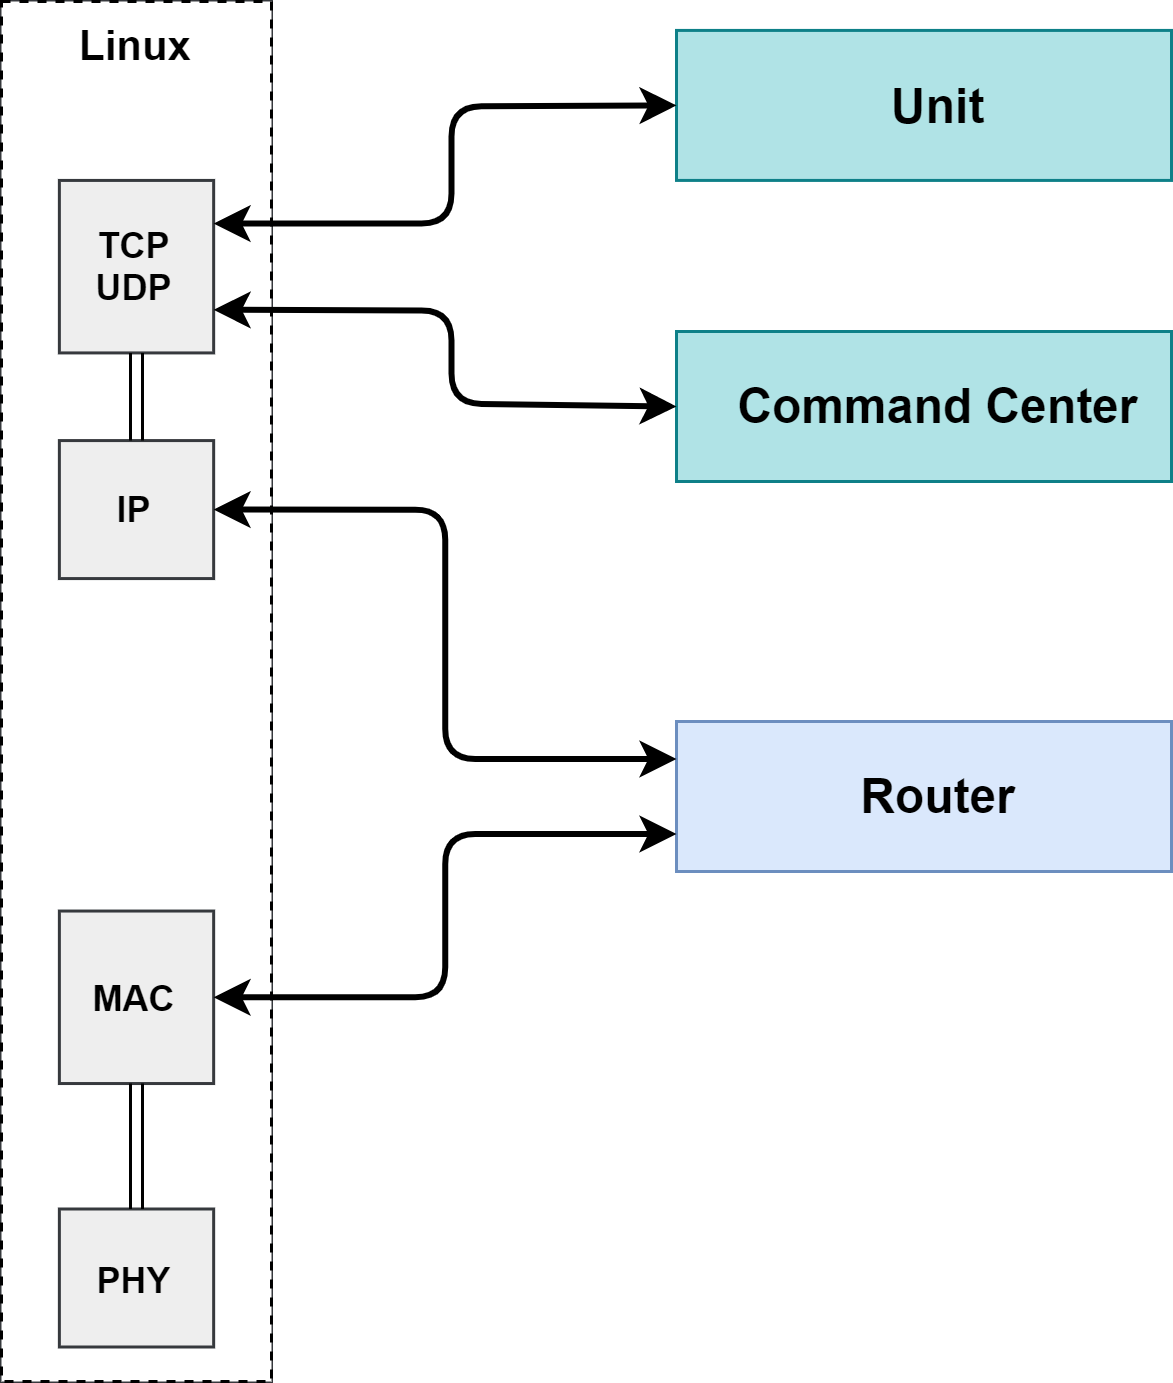
\includegraphics[width=0.8\linewidth]{images/overall-system.png}
    \caption{Overall System}
    \label{fig:overall-system}
\end{figure}

Figure \ref{fig:overall-system} shows the overall \acrshort{caian} system modules.

Unit or Command Center are applications that communicate directly with the TCP/UDP standard OS interface.
You would only use unit or command center on one device.
They are not aware of the router that sits on the bottom, this means they should work on localhost, which we already do for testing purposes to isolate system modules.

The router sits in the bottom, it's backward compatible with the Linux kernel network stack design, this means that programs in the application layer won't change when using the router.
The router takes packets going out of the system, and encrypts the packet and wraps it with our own headers and decides the forwarding of the packet.
Then the router puts back the packet in the \acrshort{mac} layer, so it's sent to the destination.

In the testing environment, as we will detail in chapter \ref{ch:system-testing}, we will isolate routers in each container with its own network stack, and create either a unit or command center program depending on the node type.

\section{The Router}
Routing is the process of filling the forwarding tables, while forwarding is the process of taking a packet and deciding the destination from the forwarding table.
The router is the main component of the project, the rest are applications that show the effectiveness of the router.
The router is backward compatible with Linux's standard network stack and works completely in the user space.

The router enables all programs and kernel modules that communicate with the \acrshort{ip} layer to run over an ad-hoc network transparently without changing any line of code.

\subsection{Functional Description}
The router takes the packet after wrapping the TCP/UDP/ICMP with IP headers, and wraps it with its packet \acrfull{zid} for interzone forwarding and encrypts the whole packet.
The router also encrypts all packets including control packets before them leaving the device.
This stops any device that doesn't share the same credentials from participating in the network and ensures the security of the communications.

The router exchanges control packets to build the topology that may be used for forwarding when a packet is available.

The router provides unicast, multicast and broadcast services to the upper layers based on \acrshort{ip} address patterns.

\subsection{Modular Decomposition}
Figure \ref{fig:router-modules} shows the modules of the router in detail.

\begin{figure}[!htb]
    \centering
    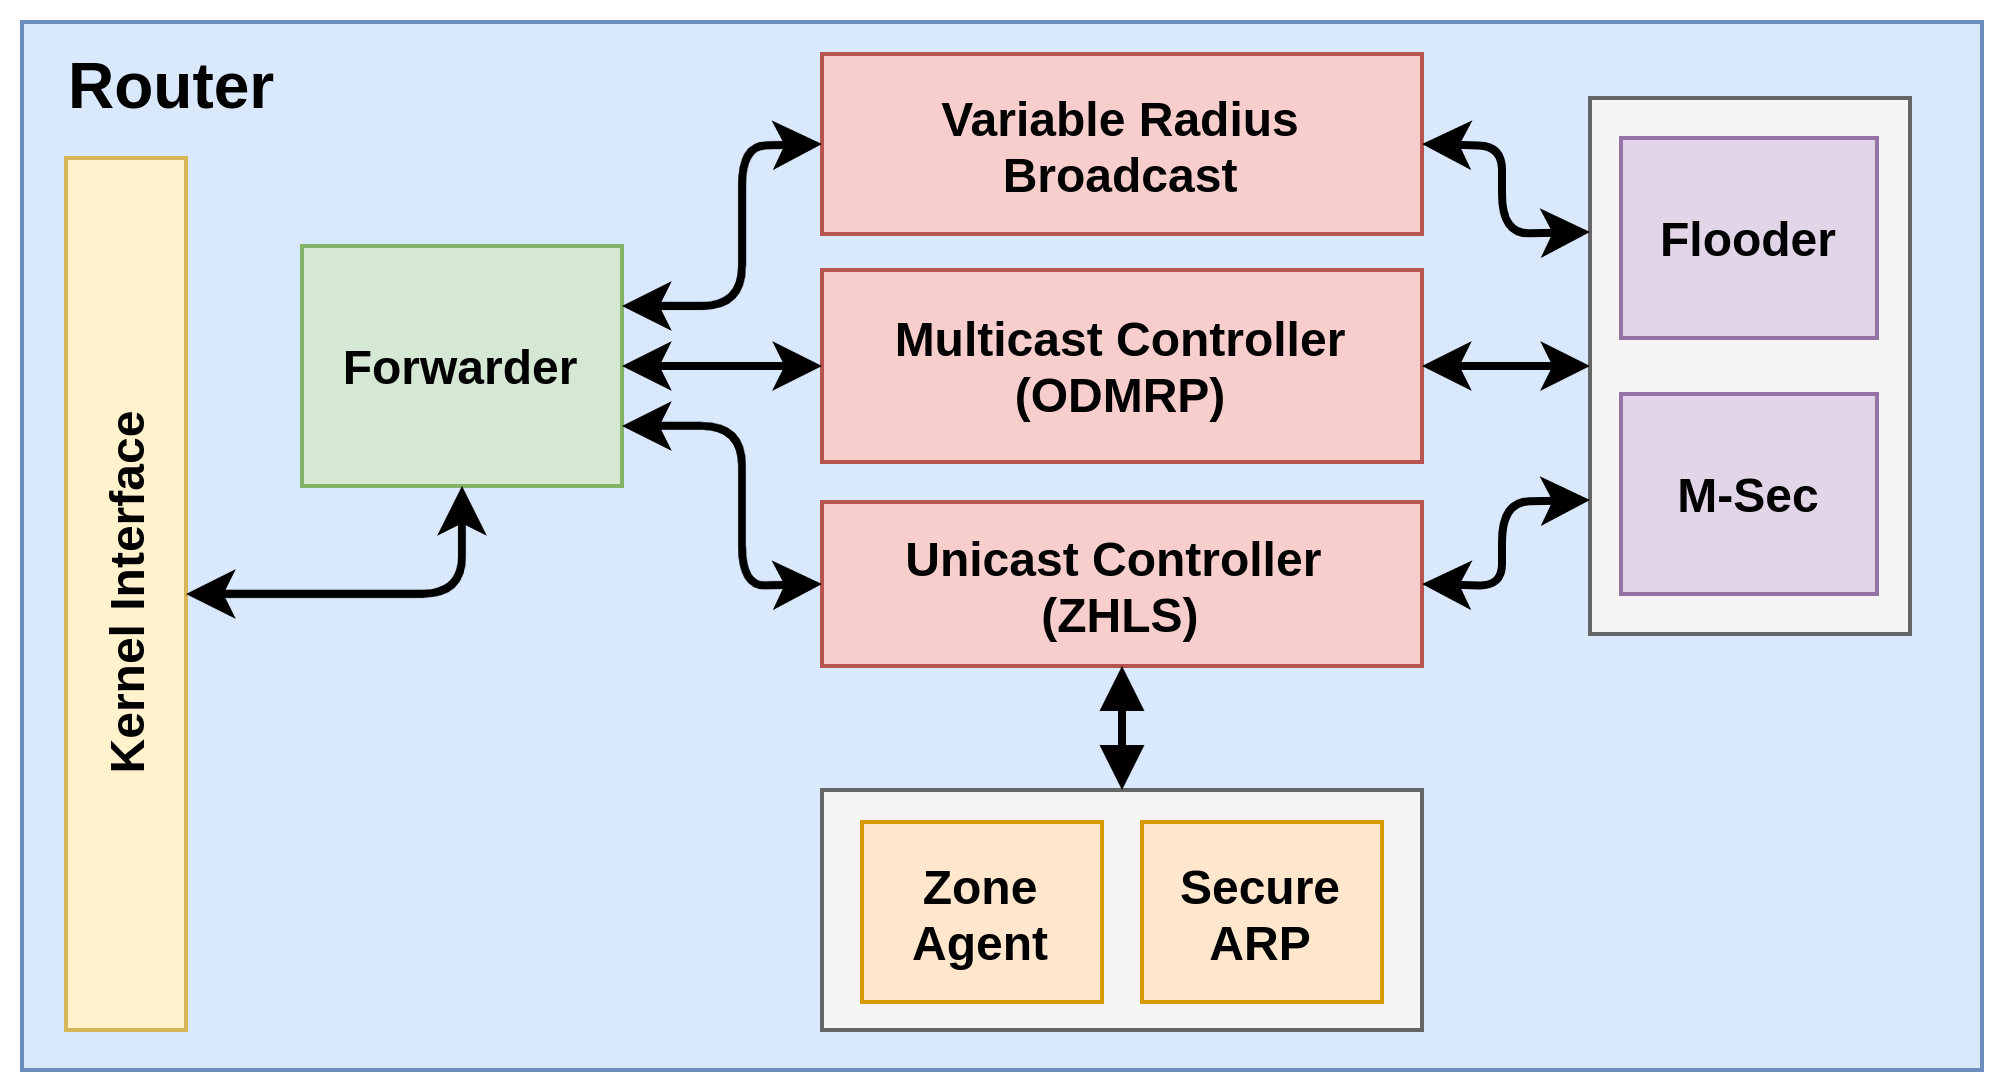
\includegraphics[width=14cm]{images/router-modules.png}
    \caption{The Router Modules}
    \label{fig:router-modules}
\end{figure}

Broadcast routing implements a new protocol we introduced called ``Variable Radius Broadcast'' (VRB), which limits the broadcast to a given geographical radius.
Unicast routing implements the ``Zone Hierarchical Link State Routing'' (\acrshort{zhls}) protocol, which solves the scalability requirements for the routing.
Multicast routing implements the infamous protocol ``On Demand Multicast Routing'' (ODMRP) protocol.

All the three routing protocols are implemented in the control plane.
They fill different kinds of forwarding tables suited for each protocol.

In the forwarding (data) plane there is the forwarder which is a complex module that takes packets leaving and entering the device and either forwards them or injects them back based on the 3 protocols' forwarding tables and has channels with the control plane to kick reactive routing decisions, like finding a zone for destination or starting the process of sending join query messages for ODMRP.

\subsubsection{Kernel Interface} 
The router reads and writes packets from the kernel in 3 ways:
\begin{itemize}[itemsep=1pt, topsep=5pt]
    \item Netfilter Queue: Used to steal packets from the kernel. They were designed in mind for firewall and deep-packet-inspections applications, but it suited our use case. The kernel gives us each packet leaving the device, and we drop them and deal with them ourselves and send it to the device driver.
    \item Packet Sockets: Used to read/write packets at the device driver, writing to it send a packet out the device.
    \item Raw Sockets: Used to inject packets into the \acrshort{ip} layer after receiving them from the 
\end{itemize}

\subsubsection{Forwarder}

The forwarder constitutes our data plane. It is where all the data packets pass and get routed. The forwarder listens to packets coming from the \acrshort{ip} layer and packets coming from the \acrshort{mac} layer. Packets coming from the \acrshort{ip} layer are packets originating at the current node, while packets coming from the \acrshort{mac} layer are packets arriving from other nodes, either addressed to the current node or to another destination. The forwarder is responsible for controlling the flow of those data packets. Figure \ref{fig:forwarder-data-flow} shows how the data flows through the forwarder.

\begin{figure}[!htb]
    \centering
    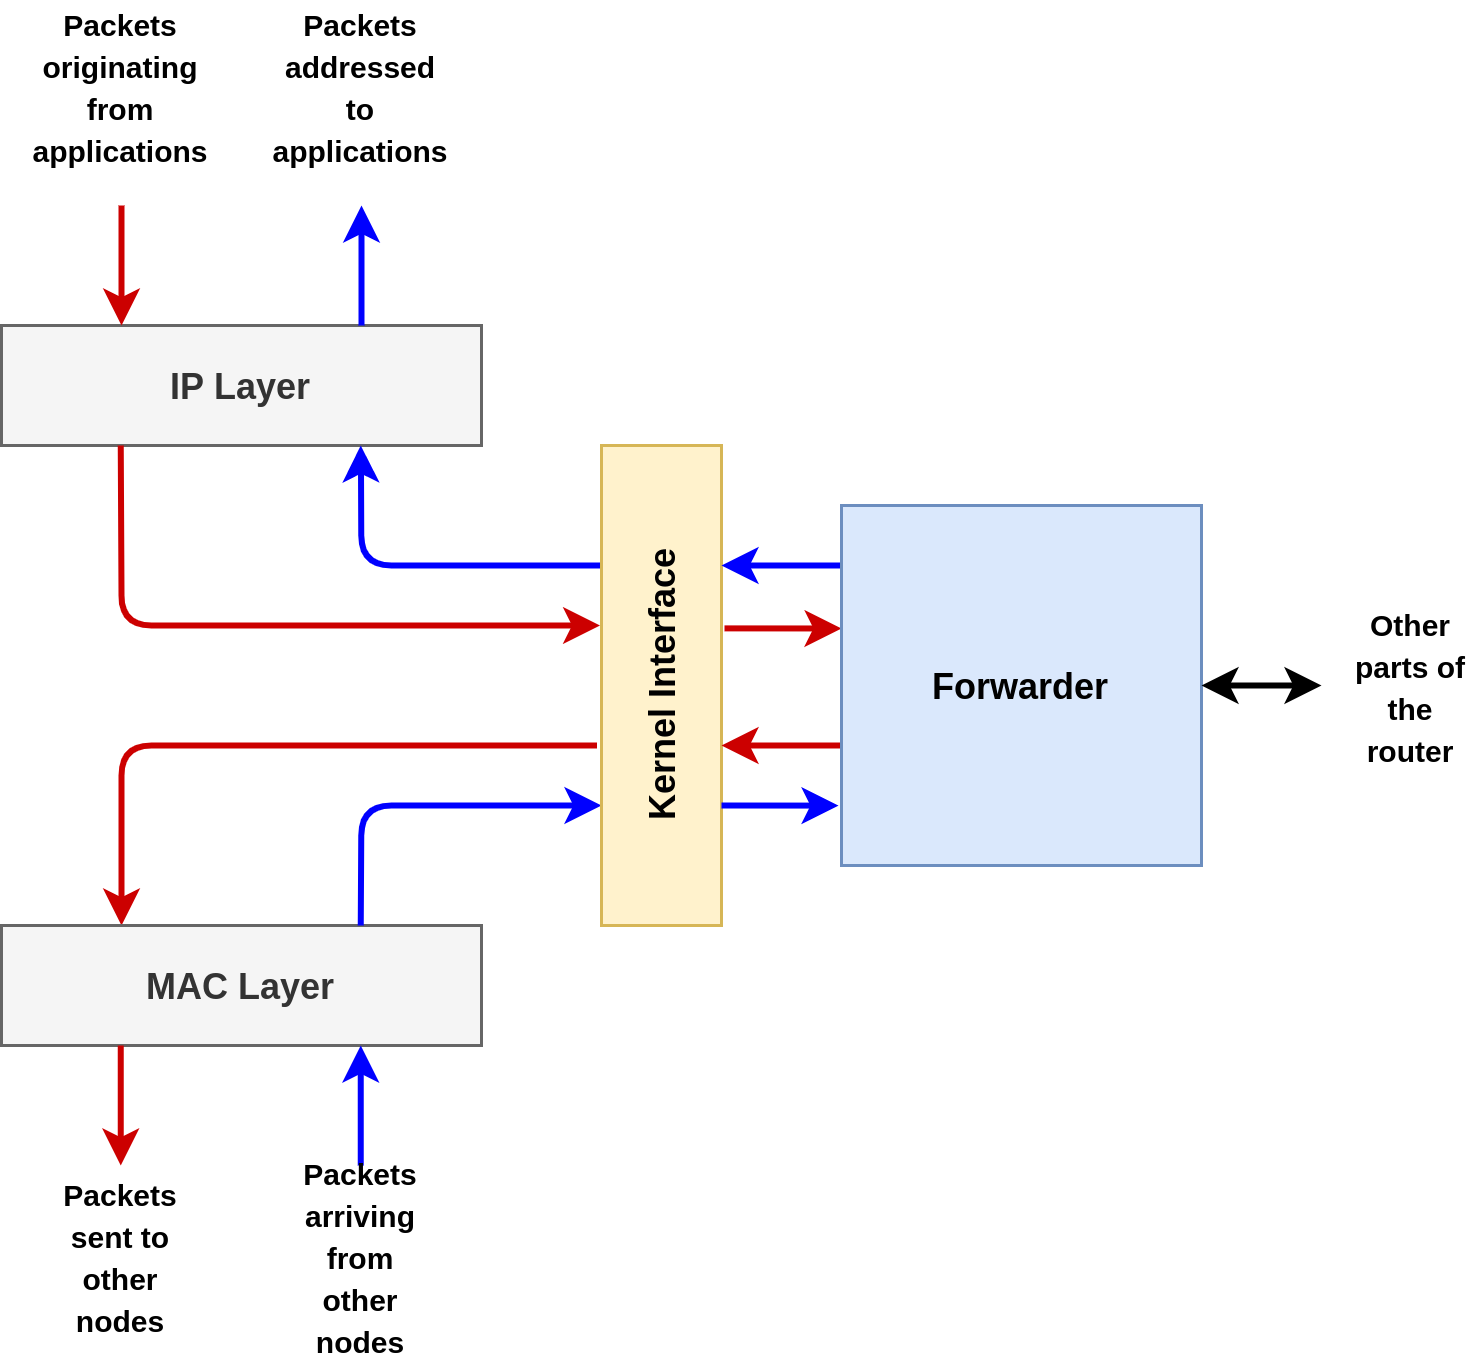
\includegraphics[width=0.9\linewidth]{images/forwarder-data-flow.png}
    \caption{Data Flow Through the Forwarder}
    \label{fig:forwarder-data-flow}
\end{figure}

When the forwarder receives data from the \acrshort{ip} layer, it first checks the type of routing required for the \acrshort{ip} packet depending on the destination \acrshort{ip} address, which can be unicasting, multicasting, or broadcasting:
\begin{itemize}[itemsep=1pt, topsep=5pt]
    \item \textbf{Unicasting}
    \begin{itemize}[itemsep=1pt, topsep=5pt]
        \item The destination zone is found through the unicast controller.
        \item A \acrshort{zid} header is constructed and prepended to the packet.
        \item The next hop is determined through the unicast forwarding table constructed by the unicast controller.
        \item The packet is encrypted and send to the next hop through the \acrshort{mac} layer.
    \end{itemize}
    \item \textbf{Multicasting}
    \begin{itemize}[itemsep=1pt, topsep=5pt]
        \item The next hop is determined through the multicast forwarding table constructed by the multicast controller.
        \item The packet is encrypted and send to the next hop through the \acrshort{mac} layer.
    \end{itemize}
    \item \textbf{Broadcasting}
    \begin{itemize}[itemsep=1pt, topsep=5pt]
        \item The packet is encrypted and sent through the variable radius broadcast handler.
    \end{itemize}
\end{itemize}

The forwarder uses different listeners to receive unicast, multicast, and broadcast packets from the \acrshort{mac} layer. The packets are differentiated using a unique ethertype used by the forwarder for each packet type. 

When the forwarder receives a unicast packet from the \acrshort{mac} layer, it decodes, decrypts and validates the \acrshort{zid} and \acrshort{ip} headers. The forwarder then checks whether the current node is the destination of the packet. If so, the packet is sent to the \acrshort{ip} layer. Otherwise, the forwarder checks if the destination node lies within the current zone's node through the \acrshort{zid} header. If it does, the forwarder checks the unicast forwarding table for the next hop for the destination node. Otherwise, the forwarder checks the unicast forwarding table for the next hope for the destination zone. The \acrshort{ip} header is then reconstructed to update the TTL and checksum, and the packet is forwarded to the next hop though the \acrshort{mac} layer. An interesting case is when a packet reaches its destination zone, but the forwarder cannot find the destination node in its zone. This may occur due to the mobility of the nodes, as the node may have left the zone after the packet was sent from the source. In this case, the forwarder uses the unicast controller to find the new zone of the destination, and reconstructs the \acrshort{zid} header with the new destination zone.

When the forwarder receives a multicast packet from the \acrshort{mac} layer, it decodes, decrypts and validates the \acrshort{ip} header. The forwarder then checks to see whether the current node is a member of the destination multicast group. If so, the packet is sent to the \acrshort{ip} layer. Regardless of whether the current node is a member, the packet may need to get forwarded according to the structure of the multicast mesh. The forwarder checks if it should forward the packet using the multicast forwarding table. If it should, it reconstructs the \acrshort{ip} header to update the TTL and checksum, and the packet is forwarder to the next hop.

\subsubsection{Variable Radius Broadcast (VRB)}
Research in ad-hoc routing gave most of its attention to unicast protocols, while broadcast and multicast were left in the dark.
Broadcasting in infrastructure networks uses the subnetting mechanism to limit the broadcasting and put boundaries, while this is most effective to decide who participates in broadcasting, but this is not applicable to ad-hoc networks because there are no subnets otherwise moving devices will be assigned different IPs each time they change cluster and this will disrupt applications logic and break the backward compatibility.

Given that \acrshort{zhls} already requires geographical locations to be maintained and shared, we figured out a way to put boundaries on the broadcasting using the current location of each device.

The protocol is simple, you know which zone you are in, when some device wants to broadcast a message it will put the broadcasting radius in the lowest byte of the destination \acrshort{ip} while setting the rest of the bits to 1.
when a device receives a broadcast a message it will check the src zone and the radius and its zone and calculates the radius between its zone and the src zone, if the calculated radius is bigger than the given radius (in the destination \acrshort{ip}) it won't forward the packet anymore otherwise it floods the message.

\subsubsection{Flooder}
Flooder is a component of any routing system that distributes every incoming packet via every outbound connection except the one from which it originated. Because \acrshort{caian} uses wireless channels as a physical layer to suit the nature of tactical teams on battlefields, and because wireless networks are broadcast by their inherent nature, this implies two important aspects in our flooding approach implementation:

\begin{itemize}[itemsep=1pt, topsep=5pt]
    \item There is no need to figure out which outgoing connection the incoming packet should be sent to; simply broadcast it.
    \item The need for a flood control method in order to avoid transmitting duplicate packets and endless recycling of the same packet.
\end{itemize}

Because \acrshort{caian} uses a zone-based routing approach for unicasting, we needed to manage the flooding area, therefore we built two flooders: a zone flooder and a global flooder. The zone flooder is primarily used to flood intrazone LSR control messages, whereas the global flooder was used by the unicast algorithm to flood interzone LSR control messages, and it was also used by the multicast algorithm.

Before flooding any packet, it must contain a \acrshort{zid} header (not required in global flooder) and a flooding header that is shown by Figure  \ref{fig:flood-header}. 

\begin{figure}[!htb]
    \centering
    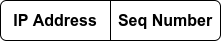
\includegraphics[scale=1]{images/flood_header.png}
    \caption{Flooding Header}
    \label{fig:flood-header}
\end{figure}

The header fields are as follows:
\begin{itemize}[itemsep=1pt, topsep=5pt]
    \item \textbf{\acrshort{ip} address:} The \acrshort{ip} address of the sender.
    \item \textbf{Seq Number:} The sequence number of that packet from that source.
\end{itemize}

Seq. number is used to control the packet flooding in the network and to prevent recirculation of the same packet indefinitely. So for any router to accept an incoming packet and flood it to all neighbors, it must satisfy three conditions:

\begin{itemize}[itemsep=1pt, topsep=5pt]
    \item It must not be flooded by the receipt router itself. 
    \item It must be flooded by a router that exists in the receipt router zone.
    \item It must have a sequence number that is higher than the latest one stored for that source.
\end{itemize}

It is obvious that the second condition is only required by the zone flooder.

According to the preceding definition, each router must keep a sequence number for each other router in the zone (or the network in the case of global flooding) that has the value of the sequence number attached with the most recent packet from that source. Each entry in the preceding flooding table has a timer connected to it in addition to the sequence number. Once the timer goes off, the entry must be deleted immediately. This timer will allow accepting packets from a router that has gone down for whatever reason and reset its sequence number to zero.

\subsubsection{M-Sec}
M-Sec stands for ``MANET Security'' which is the encryption layer we introduced in the router.
It encrypts all outcoming packets (including their headers) and decrypts all incoming packets.

M-Sec uses AES256-CFB for its speed and no found vulnerabilities yet.
We didn't choose asymmetric encryption like that used in IPsec because of the problem of certificates sharing and signing, which introduces unwanted centralization which weakens the security of the whole system in case the central authority was compromised.
Also, central authorities add to the complexity of the system, which makes it harder for huge organizations like the military and any tactical teams in general to adapt to.

M-Sec uses passphrase for its key derivation, which is done using pbkdf2 with 4096 iterations and a fixed salt.
The reason to use passphrase is to integrate seamlessly with the military way of securing communications, which they have been trained to for decades.
This enables \acrshort{caian} to be a drop-down replacement for traditional radio systems without more training.

When we encrypt a packet, we encrypt each header on its own, this enables quick decryption for the needed header to decide its destination in the forwarding plane and in case we need to update the header's data like TTL and needed to recalculate the checksum, no need to encrypt the whole packet.

Using CFB mode enables the packet to be encrypted without increasing its size because it's a stream mode.
It was also chosen among other stream modes because of its capability to detect tampering with the packet, in case someone changed one bit the whole stream will change completely which will be detected easily either by the \acrshort{ip} header checksum or version or TCP/UDP/ICMP length or checksum or the application layer.
This provides authentication besides confidentiality.

\section{Unicast Controller}
\subsection{Functional Description}
The unicast controller is in charge of one-to-one transmission between two network nodes; that is, one sender and one receiver, each with an \acrshort{ip} address. At every node, it creates a forwarding table, which includes the best next-hop to forward a packet to for each possible destination. Collectively, this constitutes finding a path from every possible source to every reachable destination. As indicated in the preceding section, we believe \acrfull{zhls} is one of the best hybrid unicast protocols for this task. As a result, we chose it as our unicast routing protocol.

\subsection{Modular Decomposition}

\begin{figure}[!htb]
    \centering
    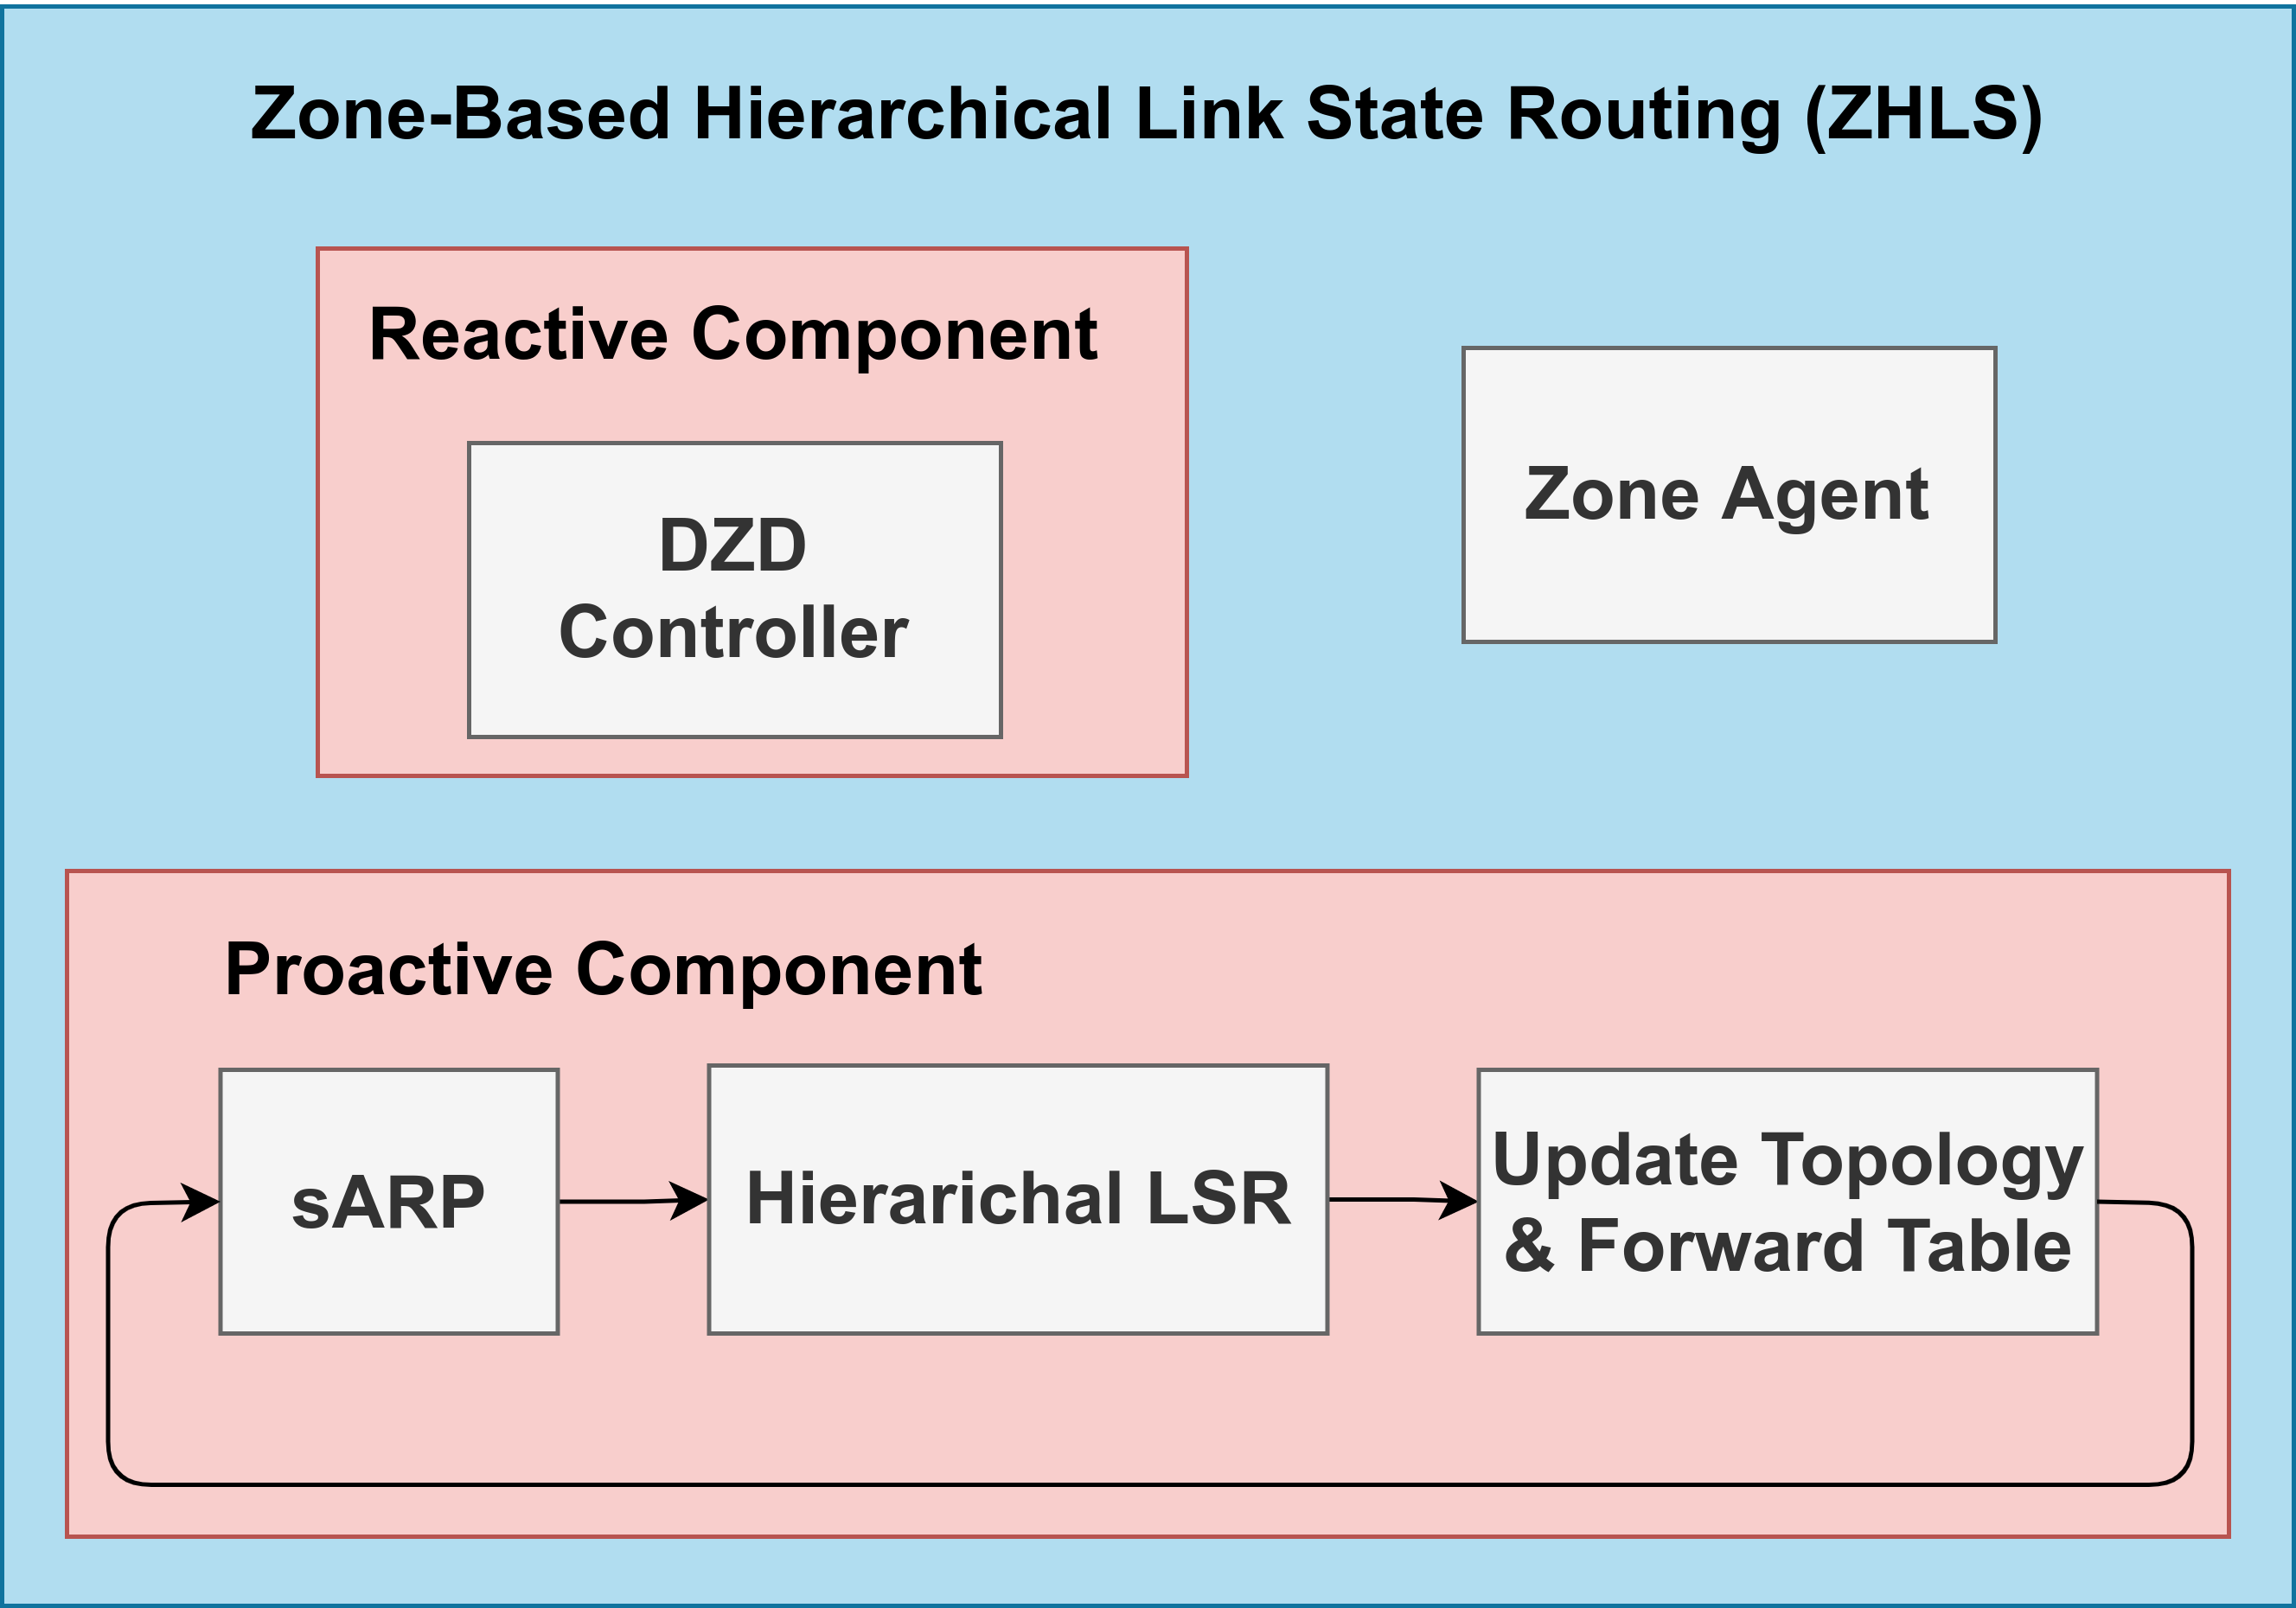
\includegraphics[width=\linewidth]{images/zhls-modules.png}
    \caption{\acrshort{zhls} Modules}
    \label{fig:zhls-modules}
\end{figure}

\acrfull{zhls} may be divided into proactive and reactive components due to the fact that it is a hybrid routing protocol. In addition, there is a module that is in charge of zone administration. \acrshort{zhls} modules can be show in Figure  \ref{fig:zhls-modules} 
The proactive component of the \acrshort{zhls} is the component that is repeated on a regular basis to gather and store up-to-date routing information about the topology and state of zones. It does this by following three consecutive protocols: collecting data about neighbor nodes and zones which is done using Secure ARP protocol, flooding this information over the network using LSR packets, and updating the hierarchical topology and forward table with the flooded information. This procedure is done on a regular basis to maintain the routing information updated. 
The reactive component of the \acrshort{zhls} is the component that is responsible for discovering the destination zone as soon as data is ready in the source and the destination \acrshort{ip} doesn't exist in the source forwarding table (the destination is in a different zone). The protocol that is used for this task is called Destination Zone Discovery (DZD). 
Finally, the Zone Agent module is in charge of managing the zones' regions and locations. It splits the whole globe into a series of variable-sized zones and uses the position of each router to determine which zone it is in.

\subsubsection{Zone Agent}
\qquad In \acrshort{zhls}, the map is divided into zones of a fixed size. In our implementation, we took it one step further and designed a variable-size zone scheme. Each zone is defined by its Cartesian coordinates, x and y. The size of each zone depends on the number of bits allocated to store the x and y coordinates, what we call the ZLength. The maximum ZLength is 16 bits, which gives the smallest zone size of 1.223 x 1.221 km\textsuperscript{2}. Different nodes may have different views of the world depending on their ZLengths as illustrated by Figure \ref{fig:zlength}. For example, if node A uses a ZLength of 14, node B uses a ZLength of 15, and node C uses a ZLength of 14, then what node A perceives as one zone is perceived as 4 zones by node B and 16 zones by node C.

\begin{figure}[!htb]
    \centering
    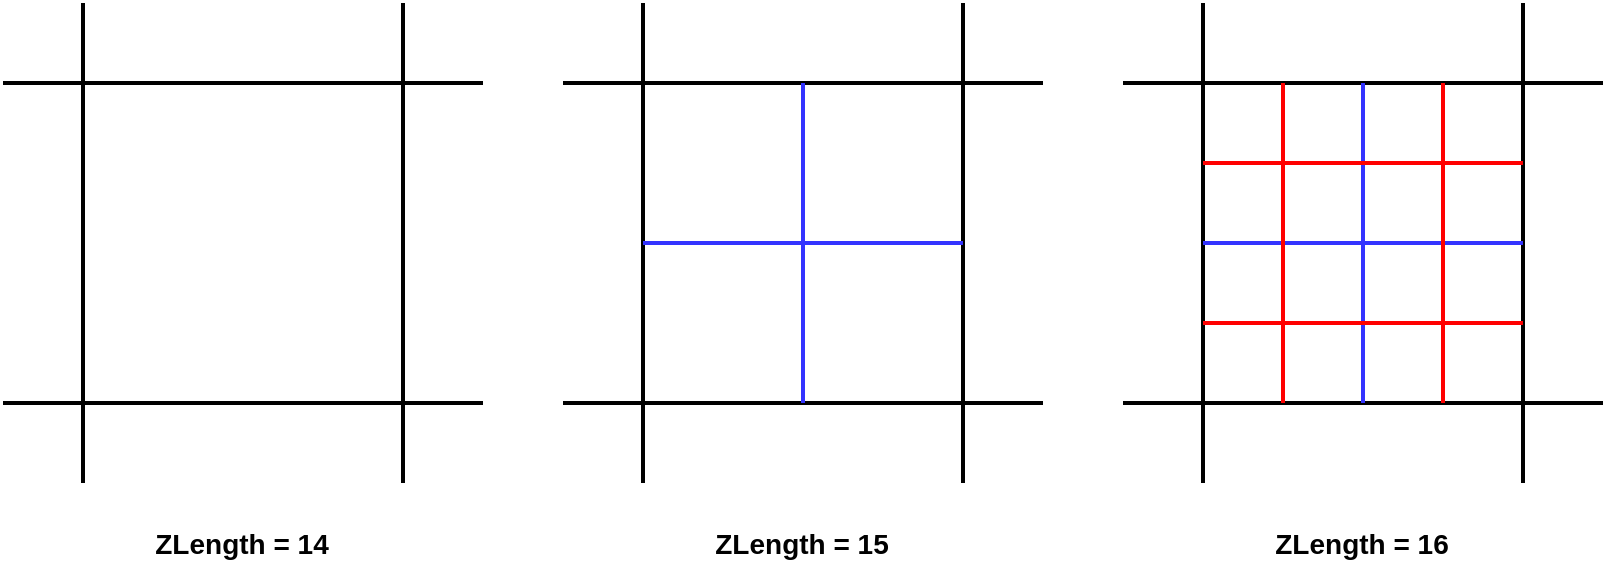
\includegraphics[width=\linewidth]{images/zlength.png}
    \caption{Zones as Perceived by Node of Different ZLengths}
    \label{fig:zlength}
\end{figure}

The zone agent connects to a GPS device using a Unix socket, and uses it to continuously read the node's latitude and longitude. The latitude and longitude are mapped from degrees to 16-bit integers to calculate the x and y coordinates. Afterward, the ZLength most significant bits of the coordinates are concatenated to form the \acrfull{zid}. If the zone agent detects that the zone is changed, it informs other submodules (subscribers) to take appropriate actions according to their logic.

\begin{figure}[!htb]
    \centering
    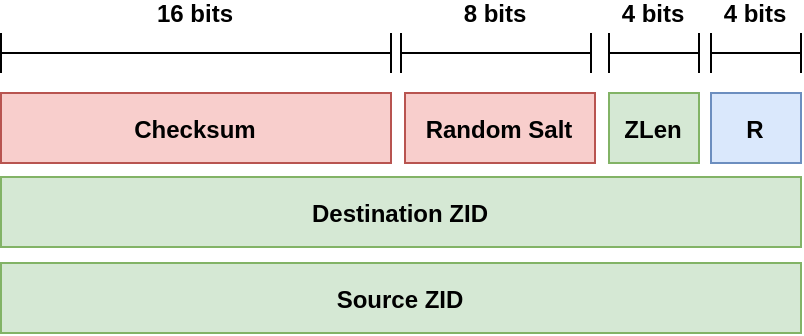
\includegraphics[width=0.8\linewidth]{images/zid.png}
    \caption{\acrshort{zid} Header}
    \label{fig:zid}
\end{figure}

The zone agent keeps track of the current zone of the node for other submodules to use. It also provides some utilities to calculate distances between zones, check if two zones are intersecting (as they may have different ZLengths), check if two zones are exactly the same, and calculate the area of a zone (which is used by Variable Radius Broadcasting). Since it holds the information of the node's current zone, other submodules use it to create \textbf{\acrshort{zid} Headers}. In our implementation of \acrshort{zhls}, a \acrshort{zid} Header is prepended to most control and data packets. It contains information about the source and destination zones, as shown by Figure \ref{fig:zid}. The header fields are as follows:
\begin{itemize}[itemsep=1pt, topsep=5pt]
    \item \textbf{ZLen:} The ZLength of the Source \acrshort{zid} and Destination \acrshort{zid} fields.
    \item \textbf{Destination \acrshort{zid}:} The Zone ID of the destination.
    \item \textbf{Source \acrshort{zid}:} The Zone ID of the source.
    \item \textbf{Random Salt:} Randomly added bits so that the encryption of a \acrshort{zid} header with the same source and destination nodes varies.
    \item \textbf{Checksum:} A checksum of the previous fields used to validate the \acrshort{zid} header.
\end{itemize}

\subsubsection{Secure \acrshort{arp}}
\qquad \acrfull{arp} is a protocol used in \acrshort{ip} networks to map layer-3 \acrshort{ip} addresses to layer-2 \acrshort{mac} addresses. \acrshort{arp} is vulnerable to \acrshort{mac} spoofing attacks, where someone in the network masquerades as someone else. Since \acrshort{caian} has many use cases where communications security is critical, we decided not to use the \acrshort{arp} protocol implementation in Linux. Instead, we implemented a secure version that we call Secure \acrshort{arp}.

Secure \acrshort{arp} is a simple protocol, similar to \acrshort{arp}, that is used in our system for three reasons:
\begin{itemize}[itemsep=1pt, topsep=5pt]
    \item Identify the direct neighbor hosts (or neighbor zones) of any given host.
    \item Find the \acrshort{ip} address to \acrshort{mac} address mapping for those direct neighbors.
    \item Calculate the latency for communicating with each neighbor node.
\end{itemize}
The main reason that Secure \acrshort{arp} can use encryption to secure its communications while \acrshort{arp} cannot, is that all nodes in a tactical team network can easily share a secret key. This is not the case in any \acrshort{ip} network, where the users may have no idea who else is present on the same network.

\begin{figure}[!htb]
    \centering
    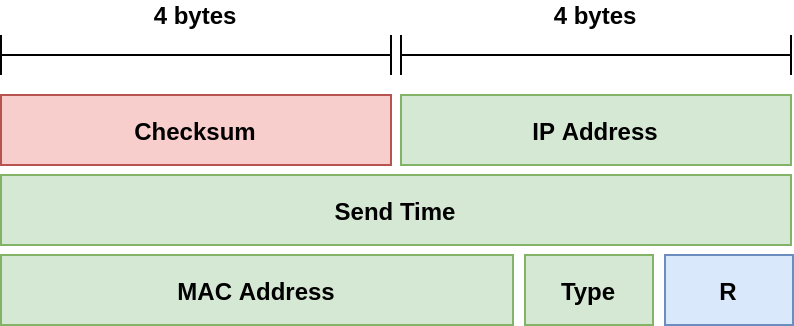
\includegraphics[width=0.8\linewidth]{images/sarp_header.png}
    \caption{\acrshort{sarp} Header}
    \label{fig:sarp-header}
\end{figure}
In Secure \acrshort{arp}, all packets consist of a \acrshort{zid} header and a \acrshort{sarp} header that is shown by Figure \ref{fig:sarp-header}. The header fields are as follows:
\begin{itemize}[itemsep=1pt, topsep=5pt]
    \item \textbf{Type:} \acrshort{sarp} packets are either a \textit{\acrshort{sarp} Request} or a \textit{\acrshort{sarp} Response}.
    \item \textbf{\acrshort{ip} address:} The \acrshort{ip} address of the sender.
    \item \textbf{\acrshort{mac} address:} The \acrshort{mac} address of the sender.
    \item \textbf{Send Time:} The time at which the packet was sent.
    \item \textbf{Checksum:} A checksum of the previous fields used to validate the \acrshort{sarp} header.
\end{itemize}

\begin{figure}[!htb]
    \centering
    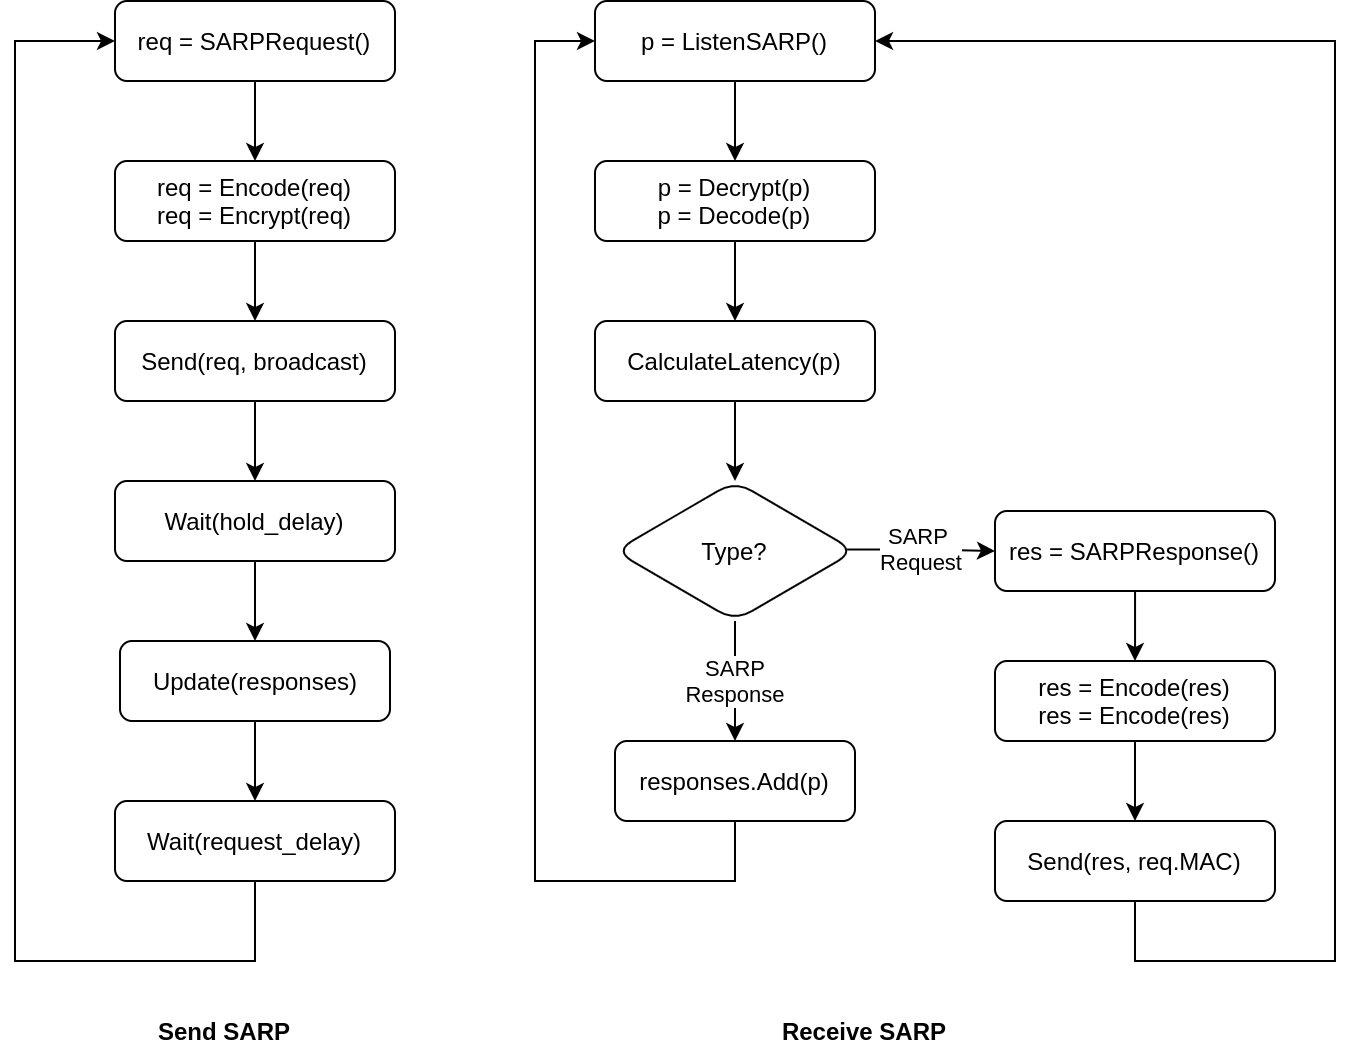
\includegraphics[width=\linewidth]{images/sarp_flowchart.png}
    \caption{\acrshort{sarp} Protocol}
    \label{fig:sarp-flowchart}
\end{figure}

\acrshort{sarp} operates through the two concurrent routines \textit{Send \acrshort{sarp}} and \textit{Receive \acrshort{sarp}} shown by Figure \ref{fig:sarp-flowchart}.
Some details are omitted for conciseness. For example, when a \acrshort{sarp} packet is received, it is actually processed in a different routine than the listening one to avoid missing a \acrshort{sarp} packet while processing a previous one.

The \acrshort{sarp} protocol operates by periodically sending and receiving \acrshort{sarp} requests and responses to find the node's direct neighbors and their information. It maintains a \textit{Neighbors Table} that contains the Node ID (\acrshort{ip} or Zone ID), \acrshort{mac} address, and most up-to-date latency of each direct neighbor node or zone. When a neighbor belongs to a different zone, it is considered as a neighbor zone rather than a neighbor node. This is determined by the \acrshort{zid} header. The \textit{Neighbors Table} is used by the Unicast Controller, as will be shown later in this chapter.

The \textit{Send \acrshort{sarp}} routine starts by creating an \acrshort{sarp} Request, encoding it into binary, and encrypting it. Afterwards, it sends the packet through the \acrshort{mac} layer to all nodes within range. The routine then waits for a hold period, giving a chance for neighbors to respond. The responses collected by the \textit{Receive \acrshort{sarp} routine} are used to update the Neighbors Table. The routine then waits again for an inter-request delay before sending the next request. The \textit{Send \acrshort{sarp}} routine also detects whether the neighbors have changed between subsequent requests by comparing hashes of the Node IDs in the Neighbors Table before and after it collects responses.

The \textit{Receive \acrshort{sarp}} routine continuously listens for \acrshort{sarp} packets. When a packet is received, it is decrypted and decoded. The latency between the current node and the sender is then calculated. If the received packet is an \acrshort{sarp} response, it is collected for the operation of the \textit{Send \acrshort{sarp}} routine. Otherwise, if is an \acrshort{sarp} Request, a response is created, encoded, encrypted, and sent through the \acrshort{mac} layer to the sender.

One last missing detail is how \textit{CalculateLatency} procedure calculates the latency information between the current node and the sender node using the send time in the \acrshort{sarp} header. To calculate the latency accurately, both nodes must be in sync. Since most tactical devices have a GPS, we assume that the GPS is used for time synchronization. 


\subsubsection{Hierarchical LSR}

\qquad Hierarchical Link State Routing (LSR) is the method through which nodes exchange information about the network. It is based on Link State Routing (LSR), in which every node constructs a connectivity graph of the whole network. However, in \acrshort{zhls} every node only maintains information about the nodes inside its own zone, in addition to zone connectivity information. It consists of two main components: Intrazone LSR and Interzone LSR.

\begin{figure}[!htb]
    \centering
    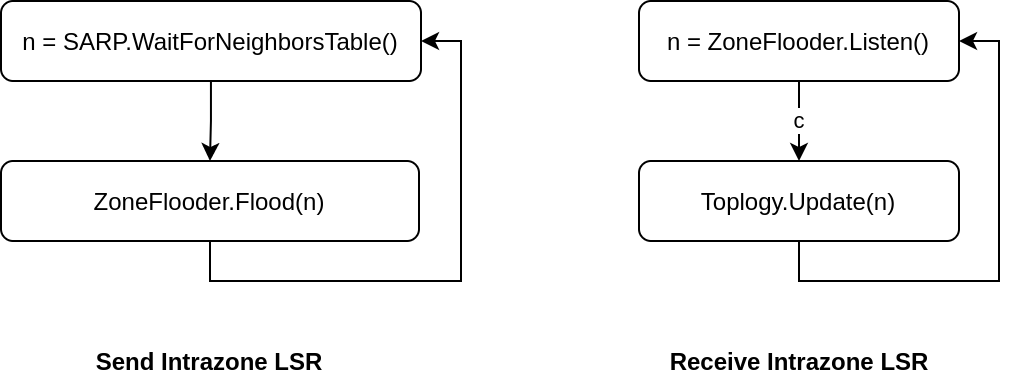
\includegraphics[width=\linewidth]{images/lsr_flowchart-intrazone.png}
    \caption{Intrazone LSR}
    \label{fig:intrazone-lsr}
\end{figure} 

In Intrazone LSR, a zone flooder is used to flood the Neighbors Table produced by Secure \acrshort{arp} every time it is updated. All nodes in a zone receive Intrazone LSR updates periodically from each other and compute connectivity information about all nodes in the zone, and the connectivity of their zone to its direct neighbor zones. Intrazone LSR is illustrated by the \textit{Send Intrazone LSR} and \textit{Receive Intrazone LSR} concurrent routines shown by Figure \ref{fig:intrazone-lsr}.

\begin{figure}[!htb]
    \centering
    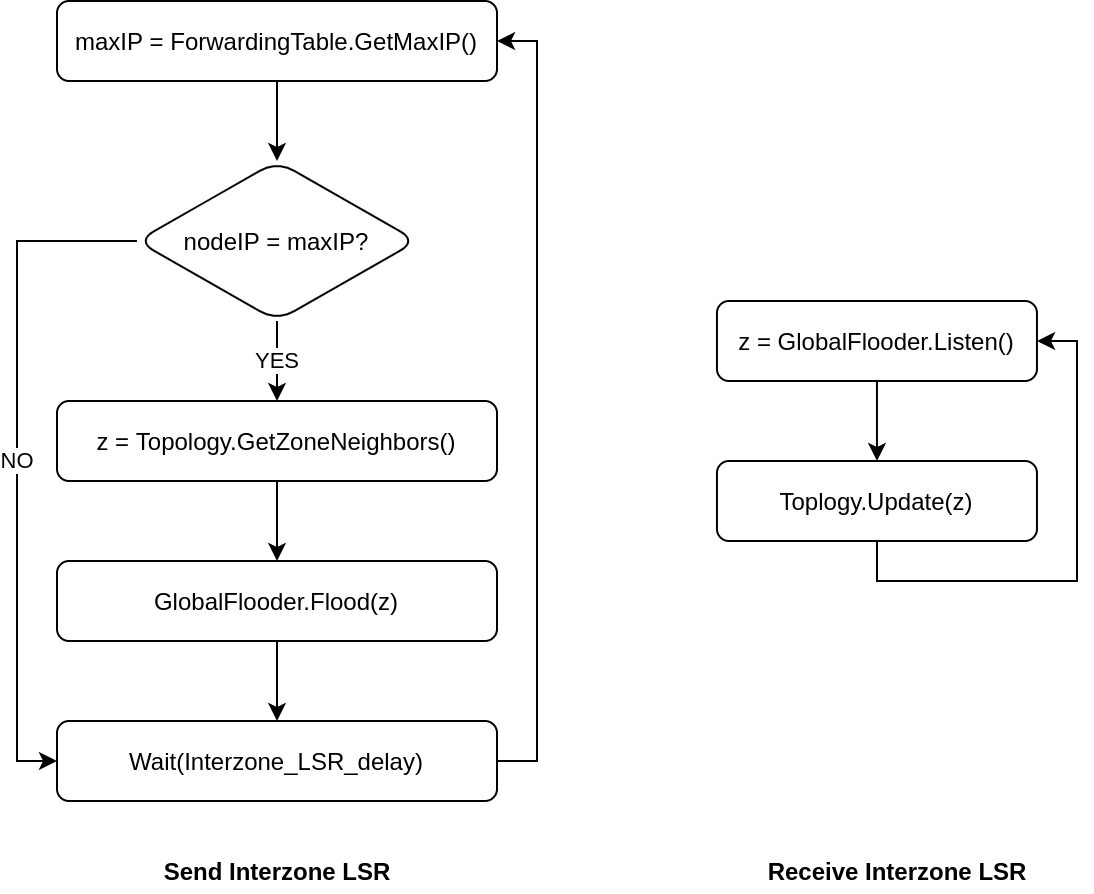
\includegraphics[width=\linewidth]{images/lsr_flowchart-interzone.png}
    \caption{Interzone LSR}
    \label{fig:interzone-lsr}
\end{figure}

In Interzone LSR, a global flooder is used to flood a special Zone Neighbors Table to all the nodes in the network periodically. A Zone Neighbors Table of a zone contains the zones that it has direct connectivity to. All nodes in the network receive Interzone LSR updates from all zones and compute connectivity information about all zones.  Interzone LSR is illustrated by the \textit{Send Interzone LSR} and \textit{Receive Interzone LSR} concurrent routines shown by Figure \ref{fig:interzone-lsr}.

A question that naturally rises in Interzone LSR is which node is responsible for sending Interzone LSR in each zone. In the original \acrshort{zhls} paper, all nodes flood Interzone LSR packets. However, this incurs a huge bandwidth overhead. In our implementation, we designed a simple scheme to avoid this. Since all nodes in a zone know the \acrshort{ip} addresses of each other (through Secure \acrshort{arp} and Intrazone LSR), they can all agree on which node has the highest \acrshort{ip} address. Hence, all nodes in a zone delegate the task of flooding Interzone LSR packets to the node with the highest \acrshort{ip} address. One might argue that with mobility and packet loss, nodes may disagree on which node has the highest \acrshort{ip} address, causing multiple ones to send Interzone LSR packets. Even though this case might occur only temporary, having two or three nodes flooding Interzone LSR packets is still better than having all the nodes in the zone do it.


\subsubsection{Hierarchical Topology Graph}
\qquad The topology graph is a major component of any proactive or hybrid routing protocol that is used to keep up-to-date routing information and is used to compute the best path from some source (usually the router itself) to any reachable destination. \acrfull{zhls} is divided into two topologies: node-level and zone-level. Consider the case when you require a path to a distant location (Interzone routing). The source node must consider both node-level and zone-level topologies and use the shortest route method on both. Aside from the memory requirements for both topologies. So we reasoned that merging both topologies into a single one with distinct types of nodes would be more efficient.\\ \\
Topology graph in \acrshort{caian} has two different type of vertices, nodes and zones as show in Figure \ref{fig:topology}. Node vertices (represented by circles) represent nodes that exist in the same zone with the router itself and each one is identified by the node \acrshort{ip}, while zone vertices (represented by squares) represent zones that are reachable from that router and each one is identified by the zone ID. 

\begin{figure}[!htb]
    \centering
    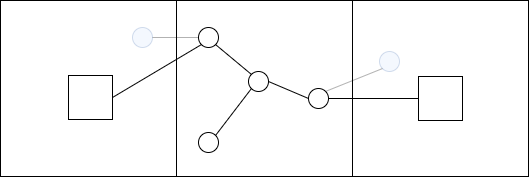
\includegraphics[width=\linewidth]{images/topology.png}
    \caption{Hierarchical Topology Graph}
    \label{fig:topology}
\end{figure} 
The following two approaches are used to keep the topology graph up-to-date for all nodes and zones routing information:
\begin{itemize}[itemsep=1pt, topsep=5pt]
    \item Periodically receives Intrazone and Interzone LSR packets as illustrated previously and uses this information to update the topology graph vertices, edges, and weights.
    \item Each vertex in the graph should have a timer attached to it (nodes and zones). Once we have received an LSR packet from that vertex, reset the timer (Intrazone LSR packets for node vertices and Interzone LSR packets for zone vertices). Remove this vertex from the topology graph instantly once the timer goes off.\\
\end{itemize} 
Keeping the topology graph up-to-date is mandatory as it will be used mainly for two important functionalities: 
\begin{itemize}[itemsep=1pt, topsep=5pt]
    \item Find the shortest paths by applying the Dijkstra algorithm (using latency metric) to all nodes and zones in the graph and use this information to fill the forwarding table.
    \item Find all reachable neighbor zones by applying controlled depth-first search from the router vertex till reaching zone vertices and use this information to apply zone-level broadcasting, which is much more efficient than normal flooding.
\end{itemize}

\subsubsection{Destination Zone Discovery}
Destination Zone Discovery (DZD) is a major module in  \acrfull{zhls}. Consider the case when the source node require a path to a node that is outside its zone (Interzone routing). The first step is to discover the zone of the required destination. 

Destination Zone Discovery (DZD) protocol has two types of control messages that control the searching process: DZD Request which is sent using zone-level broadcasting by the router that want to discover the destination zone and DZD Response which is sent using normal unicasting from the node that know the destination zone to the source node which its zone was already stored in the DZD Request header. 

DZD Request control message must contain two headers: 
\acrshort{zid} header which has the following fields:
\begin{itemize}[itemsep=1pt, topsep=5pt]
    \item \textbf{Src Zone:} The zone ID of the source node which will be used later to send the DZD Response to.
    \item \textbf{Dst Zone:} The zone ID of the neighbor zone to the source zone which is the DZD Request will be sent to.
\end{itemize} 

And DZD Request Header which has the following fields as show in Figure \ref{fig:dzd-request}:
\begin{itemize}[itemsep=1pt, topsep=5pt]
    \item \textbf{Src \acrshort{ip}:} The \acrshort{ip} of the source node which will be used later to send the DZD Response to.
    \item \textbf{Required Dst \acrshort{ip}:} The \acrshort{ip} of the destination node which it's required to know its zone.
    \item \textbf{Visited Zones:} Array of all zones that the DZD Request message has already gone through. This array is used to prevent recirculation of the same message indefinitely. 
\end{itemize} 

\begin{figure}[!htb]
    \centering
    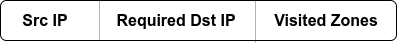
\includegraphics[scale=0.7]{images/dzdrequest_header.png}
    \caption{DZD Request Header}
    \label{fig:dzd-request}
\end{figure} 

The reachable neighbor zones are found using depth-first search on the hierarchical topology graph, and a copy of the DZD Request message is sent to each of them once the DZD Request message is generated using the preceding headers. Each zone will repeat the process until the destination zone is discovered.

The first node that receive the DZD Request message at the destination zone will stop broadcasting DZD Request message and start to form DZDResponse message using \acrshort{zid} header which contains:
\begin{itemize}[itemsep=1pt, topsep=5pt]
    \item \textbf{Dst Zone:} The zone ID of the destination zone which, in this case, the zone of the source node that started broadcasting DZD Response message.
\end{itemize} 

And DZD Response Header which has the following fields as show in Figure \ref{fig:dzd-response}: 
\begin{itemize}[itemsep=1pt, topsep=5pt]
    \item \textbf{Dst \acrshort{ip}:} The \acrshort{ip} of the destination node which, in this case, the source node that started broadcasting DZD Response message.
    \item \textbf{Required Dst \acrshort{ip}:} The \acrshort{ip} of the destination node which it's required to know its zone.
    \item \textbf{Required Dst Zone ID:} The destination zone ID which the source node was looking for it.
\end{itemize} 

\begin{figure}[!htb]
    \centering
    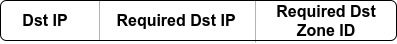
\includegraphics[scale=0.7]{images/dzdresponse_header.png}
    \caption{DZD Response Header}
    \label{fig:dzd-response}
\end{figure} 

Using the Dst \acrshort{ip} in DZD Response Header and Dst Zone in \acrshort{zid} Header, DZD Respone packet can be unicasted to the original source that sent DZD Request message. Each node along the path of DZD Respone and the original source itself cache the destination zone for upcoming messages.

The original source can transmit all data buffered to that destination after receiving the DZD Response message. If the search fails, it will be repeated three times, each time after a certain amount of time, until the target zone is found, otherwise it will be announced as a failure and all stored packets for that destination will be discarded.

\section{Multicast Controller}
\subsection{Functional Description}
The multicast controller is in charge of many-to-many transmission between network nodes; that is, multiple senders and multiple receivers, each with an \acrshort{ip} address. At every node, it creates a Multi-Forwarding table, which includes the best next-hops to forward a packet to for each possible multicast group. Collectively, this constitutes by periodically sending control packets join query and join replies and filling tables in every. As indicated in the preceding section, we believe On-Demand Multicast Routing Protocol (ODMRP) is one of the best multicast protocols for this task. As a result, we chose it to be our multicast routing protocol.

\subsection{Modular Decomposition}

\begin{figure}[!htbp]
    \centering
    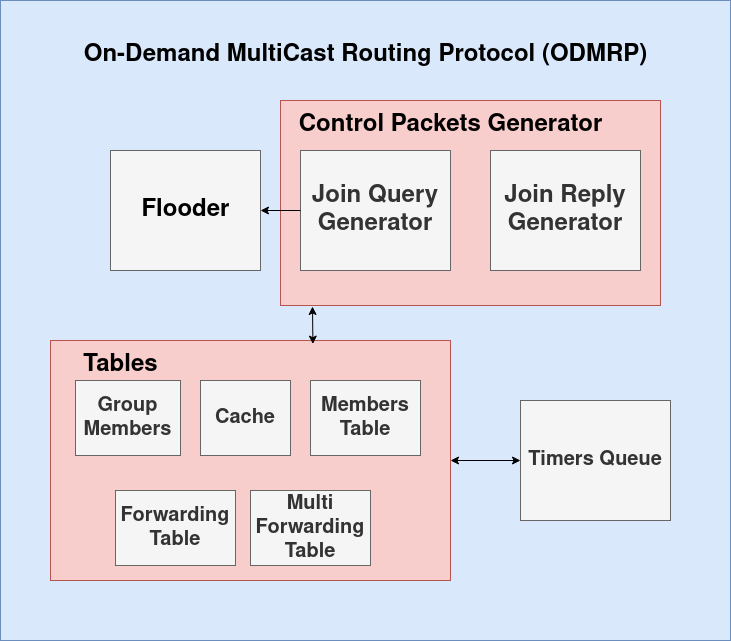
\includegraphics[width=\linewidth]{images/odmrp-modules.png}
    \caption{ODMRP Modules}
    \label{fig:odmrp-modules}
\end{figure}

On-Demand Multicast Routing Protocol (ODMRP) may be divided into two part, the control packet generator and the tables. In addition, there is a flooder module is in charge of flooding the join query packets and timers queue for deleting expired table entries from the tables. ODMRP modules can be show in Figure  \ref{fig:odmrp-modules}
\\
\subsubsection{Control Packets Generator}
Generating right control packets is critical for this protocol as ODMRP depends on the control packets for filling the tables, construct the routes and the network soft state maintenance.
This module generates two important control packets called Join Query (format illustrated in Figure \ref{fig:join-query}) and Join Reply (format illustrated in Figure \ref{fig:join-reply}).
\\
A Join Query is generated when a multicast source has packets to transmit but no route and group membership is known, a Join Query packet contains the following fields: 
\begin{itemize}[itemsep=1pt, topsep=5pt]
    \item \textbf{Dests Count:} The Number of destinations IPs.
    \item \textbf{Checksum:} It is used to validate the received control packet.
    \item \textbf{SeqNo:} Unique sequence number of the control packet.
    \item \textbf{TTL:} Time to live, which is the number of hops this packet can traverse.
    \item \textbf{SrcIP:} Source \acrshort{ip} address where the control packet is generated.
    \item \textbf{GrpIP:} Group \acrshort{ip} address of this multicast group.
    \item \textbf{PrevHop:} Mac address of the last node which has processed this packet.
    \item \textbf{DestIPs:} The destination IPs of this multicast group.
\end{itemize} 

\begin{figure}[!htbp]
    \centering
    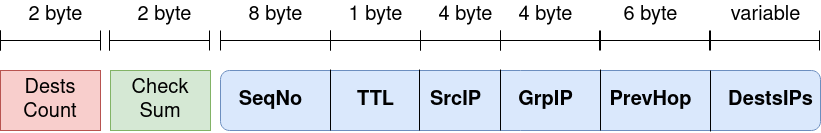
\includegraphics[width=\linewidth]{images/join-query.png}
    \caption{Join Query Packet}
    \label{fig:join-query}
\end{figure}

Join Query control packet is generated using the following:
\begin{itemize}[itemsep=1pt, topsep=5pt]
    \item \textbf{SeqNo:} Incremental value in the multicast control module,
    different for each control packet sent.
    \item \textbf{TTL:} Default time to live value in our case we set it to 100.
    \item \textbf{SrcIP:} This Node \acrshort{ip} where the join query packet is generated.
    \item \textbf{GrpIP:} Group \acrshort{ip} address of this multicast group.
    \item \textbf{PrevHop:} \acrshort{mac} of current node.
    \item \textbf{DestIPs:} The destination IPs of this multicast group \acrshort{ip}.
\end{itemize}

Then this Join Query packet is flooded using the flooder and gets updated and update the node's tables until it reaches a destination the destination node generates a Join Reply control packet which contains the following fields:
\begin{itemize}[itemsep=1pt, topsep=5pt]
    \item \textbf{Next Hops Count:} Next Hops \acrshort{mac} addresses count which equals the source IPs address count either.
    \item \textbf{Checksum:} It is used to validate the received control packet.
    \item \textbf{SeqNo:} Unique sequence number of the control packet.
    \item \textbf{DestIP:} Destination \acrshort{ip} where the Join Reply is generated.
    \item \textbf{GrpIP:} Group \acrshort{ip} address of this multicast group.
    \item \textbf{PrevHop:} Mac address of the last node which has processed this packet.
    \item \textbf{SrcIPs:} Source IPs addresses where the control packet is generated.
    \item \textbf{Next Hops:} Next Hops \acrshort{mac} addresses to reach the sources.
    \item \textbf{Cost:} Cost of this path, which equals the number of hops.
\end{itemize}

\begin{figure}[!htbp]
    \centering
    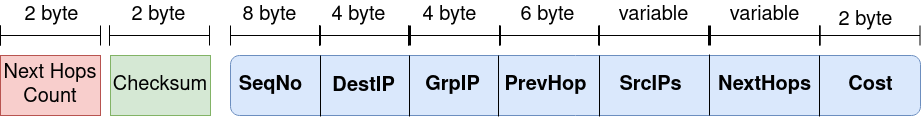
\includegraphics[width=\linewidth]{images/join-reply.png}
    \caption{Join Reply Packet}
    \label{fig:join-reply}
\end{figure}

Join Reply control packet is \textbf{generated} using the following:
\begin{itemize}[itemsep=1pt, topsep=5pt]
    \item \textbf{SeqNo:} Received join query sequence number.
    \item \textbf{DestIP:} \acrshort{ip} of the current node where the Join Reply is generated.
    \item \textbf{GrpIP:} Group \acrshort{ip} address of this multicast group.
    \item \textbf{PrevHop:} Mac address of the current node.
    \item \textbf{SrcIPs:} Filled using cache table by iterating on cache table entries and checks if the group \acrshort{ip} is equal to the group IP of this multicast group, if true it appends the source IP found in the cache table to this join reply control packet.
    \item \textbf{Next Hops:} Filled using cache table by iterating on cache table entries and checks if the group \acrshort{ip} is equal to the group IP of this multicast group, if true it appends the next hop found in the cache table to this join reply control packet.
    \item \textbf{Cost:} 1.
\end{itemize}

Then Join Reply packet is sent to the next hops addresses and gets updated and update the tables then passed to the next hops addresses until it reaches the multicast sources.

\subsubsection{Tables}
As we knew in Chapter \ref{ch:literature-survey} ODMRP are mesh based and soft state protocol, so tables play big role in ODMRP protocol to construct the mesh, forwarding group members and the routes to reach the destinations nodes.

\textbf{Group Members Table} is the table which is used to hold the multicast group \acrshort{ip} address and the corresponding destinations \acrshort{ip} addresses So a packet can be sent using only the group \acrshort{ip}, Figure \ref{fig:group-members-table-entry} represents one entry of Group Members Table, It is filled by a configuration file in the senders nodes.
\begin{figure}[!htbp]
    \centering
    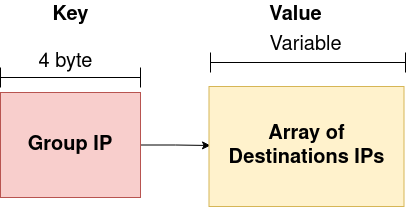
\includegraphics[scale=0.7]{images/group-members-table-entry.png}
    \caption{Group Members Table}
    \label{fig:group-members-table-entry}
\end{figure}
\\
\\
\textbf{Cache Table} is the table that holds the control packet source \acrshort{ip} and the corresponding (Sequence Number, Group \acrshort{ip}, Previous Hop and cost). And the table is used to:
\begin{enumerate}
    \item Check for control packet duplicates.
    \item Hold cost value to check if a better entry has been found.
    \item Generate and update join reply control packet.
\end{enumerate}
Figure \ref{fig:cache-table-entry} represents one entry of Cache Table.
\begin{figure}[!htbp]
    \centering
    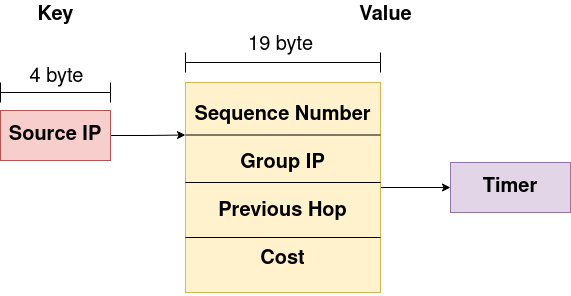
\includegraphics[width=\linewidth]{images/cache-table-entry.png}
    \caption{Cache Table Entry}
    \label{fig:cache-table-entry}
\end{figure}
\\
\\
\textbf{Members Table} is a table that holds the group IPs that the current node is a part of. This table for faster checking that the current node is a destination of a certain multicast group \acrshort{ip} address, and it gets filled the first time the node knew it is a destination of a certain multicast group \acrshort{ip} address. Figure \ref{fig:member-table-entry} represents one entry of Members Table.
\begin{figure}[!htbp]
    \centering
    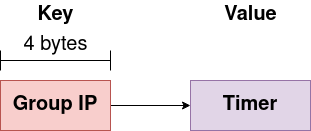
\includegraphics[scale=0.8]{images/member-table-entry.png}
    \caption{Members Table Entry}
    \label{fig:member-table-entry}
\end{figure}
\\
\\
\textbf{Forwarding Table} is a table that holds some entries, each one has a destination \acrshort{ip} address and the corresponding next hop \acrshort{mac} address and cost. It gets filled when receiving a join reply from a destination, and it is used to update the Multi Forward Table (more details in the next section \ref{sec:odmrp-protocol-flow}).
Figure \ref{fig:forwarding-table-entry} represents one entry of Forwarding Table.

\begin{figure}[!htbp]
    \centering
    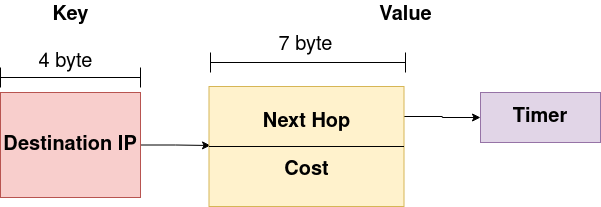
\includegraphics[width=\linewidth]{images/forwarding-table-entry.png}
    \caption{Forwarding Table Entry}
    \label{fig:forwarding-table-entry}
\end{figure}

\textbf{Multi Forward Table} is a table that holds some entries, each one has a multicast group \acrshort{ip} address and the set of corresponding next hops to reach this multicast group \acrshort{ip} destinations. It gets filled when receiving a join reply from a destination (more details in the next section \ref{sec:odmrp-protocol-flow}), and this table is used by the node router to direct the packets to reach destinations node of a certain multicast group \acrshort{ip} address.
Figure \ref{fig:multi-forward-table-entry} represents one entry of Multi Forward Table.
\begin{figure}[!htbp]
    \centering
    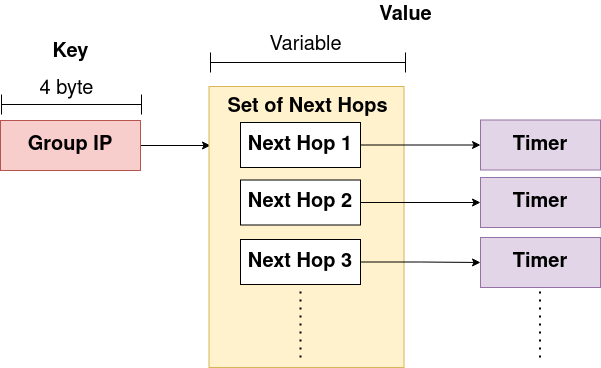
\includegraphics[width=\linewidth]{images/multi-forward-table-entry.png}
    \caption{Multi Forward Table Entry}
    \label{fig:multi-forward-table-entry}
\end{figure}
\\
\\
\\
\\
\\
\\
\subsection{ODMRP Protocol Flow}
\label{sec:odmrp-protocol-flow}
In ODMRP \cite{ODMRP}, group membership and multicast routes are formed and updated by the source on demand. When a multicast source has packets to transmit but no route and group membership is known (Multi Forward \ref{fig:multi-forward-table-entry} Table is empty), it floods an advertising control packet. This packet, named Join Query (format illustrated in Figure \ref{fig:join-query}) and it is regularly sent by the flooder to the whole network to refresh the membership information and update the routes.
\\
\\
When a node gets a Join Query packet, time to live is decreased by one, and it records the source address and the unique identifier of this control packet to its Cache Table \ref{fig:cache-table-entry} to identify duplication to construct the join reply later.
If the Join Query control packet is not a duplicate by verifying it is not a duplicate from the cache table and the Time to live is higher than zero, the cache table is updated, and it is rebroadcast.
\\
\\
When a Join Query packet reaches the multicast receiver, it adds the group \acrshort{ip} to its member table as an entry (Figure \ref{fig:member-table-entry}) so the node realizes that it is a part of this forwarding  group with a specific group \acrshort{ip} address.
\\
The destination node then generates a Join Reply control packet (format shown in Figure \ref{fig:join-reply}) with the help of the cache table to add next hops and source IPs which are filled before by the received join queries and sets the cost of the generated join reply to be one.
\\
\\
Then sends the generated join reply to the previous hops nodes, The classical ODMRP protocol floods the join replies packet until it reaches all the sources, We did an \textbf{optimization} by sending the join reply via the next hops stored in the cache and making the join reply propagated and received by only the forwarding group members and not broadcasted to any other node which are not a part of this multicast group.
\\
After generating the join reply control packet sends the join reply with the same manner by updating the source IPs, next hops, the cost, update the forwarding table \ref{fig:forwarding-table-entry} and also construct the routes by filling the multi forward table \ref{fig:multi-forward-table-entry} with the next hops \acrshort{mac} addresses corresponding to this group \acrshort{ip} address.
Updating the route in the Multi Forward Table is done by checking if the forwarding table is updated by a newly added destination \acrshort{ip} or destination \acrshort{ip} address exists but the new received join reply cost is less than the existing one. If this is true, both the forwarding table and multi forward table are updated by adding the previous hop of the received join reply to the Next hops set, using the group \acrshort{ip} as the key of the next hops.
\\
\\
This method generates a mesh of nodes with forwarding group members and routes from sources to receivers until it reaches the multicast source through chosen paths.
\\
When the node's router wants to send a multicast packet is checks if Multi Forward Table has entries using this multicast group \acrshort{ip} address as the key, and it can access a set of next hops to send the packet to them, so it can do multicasting.

\section{Command Center Client}
Command centers are responsible for the central administration and operational management of a group of units. High-end computers with strong CPUs, high power consumption capabilities, and large storage and RAM capabilities are expected to be used as command center clients. The command centers are located near the operation field and have a wide wireless range, allowing them to link to a group of troops in the field. They're assumed to have limited (or no) mobility.


\subsection{Functional Description}
Command centers in \acrshort{caian} have the ability to collect data from a collection of units, show it to the operators or unis leaders, and control these units by delivering a series of instructions.
What exactly a command center can perform is summarized briefly in the following list:
\begin{itemize}[itemsep=1pt, topsep=5pt]
\item Send audio command and command codes to a single unit.
\item Send audio commands to a group (multicast) or everyone (unlimited-radius broadcast).
\item Store all sent and received data.
\item Show old data (audio, messages, videos, sensor data)
\item Show notifications when an audio message or command code is received.
\item Show video streams as they are received from units.
\item Show a map of connected units distinguished by group color to each unit belonging to some group.
\item If sensor data isn’t received in 2 minutes, mark the unit as inactive and notify the command center operators.
\item  If a unit’s heartbeat is below a threshold, mark it as in danger and notify the command center operators.
\end{itemize} 

\subsection{Modular Decomposition}
As illustrated in Figure \ref{fig:cmd-center}, \acrshort{caian}'s command center is organized into two major modules: Daemon, which is in charge of sending and receiving data from other units in the network, and User Interface, which allows operation leaders to manage and visualize this data as well as record command audios and choose command codes that they want to send to these units.

\begin{figure}[!htb]
    \centering
    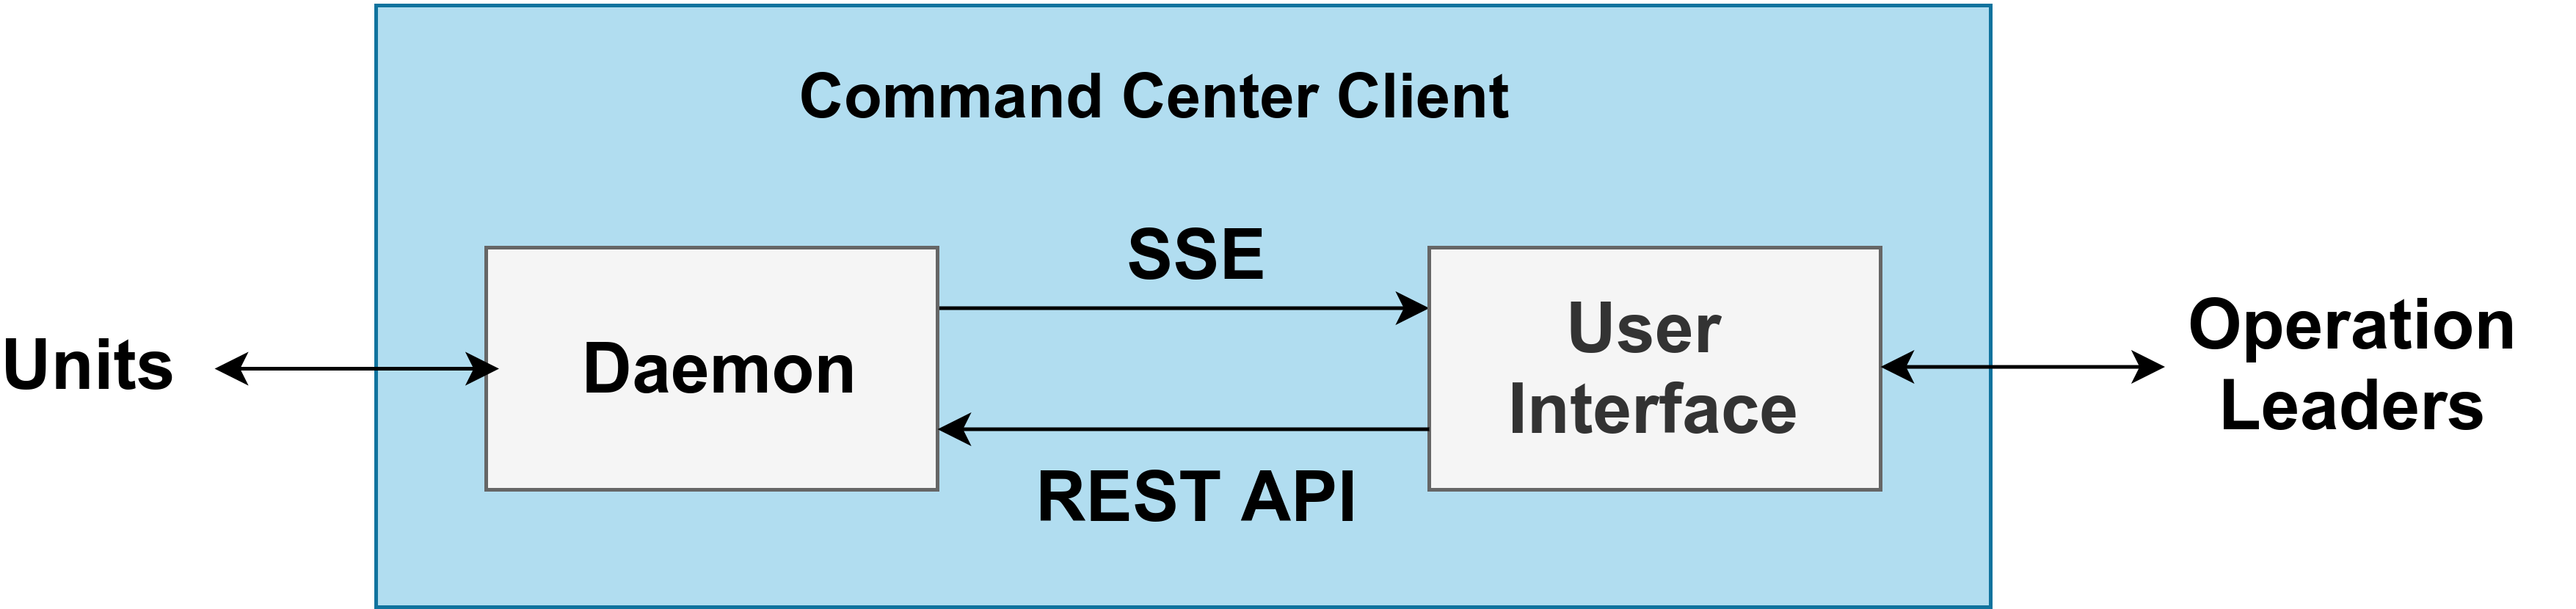
\includegraphics[width=\linewidth]{images/command-center.png}
    \caption{Command Center Client}
    \label{fig:cmd-center}
\end{figure}

Video Streamer is a submodule of both the Daemon and User Interface that will be discussed in better detail later.

\subsubsection{Daemon}
The daemon of the command center client is a highly concurrent program that runs in the background on the command center's devices. It exchanges code messages, audio messages with units, and receive sensors data and video streaming from the units through a network interface, runs a database to keep track of all sent and received data, and connects to the user interface through a \acrshort{rest}ful \acrshort{api} server.

On the network interface, the unit has two concurrent routines that listen for TCP connections and UDP datagrams. When receiving a TCP connection or a UDP datagram, the incoming data is handled in a separate concurrent routine to avoid missing connections or incoming datagrams while processing previous ones. Any data received is prepended with a byte that identifies the packet type. The packet payload is then decoded, the data is stored in the database, and the user interface is notified through \acrfull{sse}. The network interface also provides routines to send or receive packets over TCP or UDP to units, in case the command center needs to send code messages or audio messages to a unit, a group of units, or all the units. Note that all TCP and UDP data transfers are routed using our router.

The \acrshort{rest}ful \acrshort{api} server runs in a concurrent routine and provides endpoints for the user interface to collect and present stored data. In addition, it provides endpoints for the user interface to send code messages or audio messages to unit(s). All sent and received data are stored in the database. Since the database is accessed through different concurrent subroutines, mutual exclusion techniques are used to synchronize access to the database.

The main routine reads any necessary configuration or command line arguments on startup, initializes the database, then starts and orchestrates the aforementioned subroutines. Figure \ref{fig:cmd-daemon} shows a complete picture of the command center client daemon.

\begin{figure}[!htb]
    \centering
    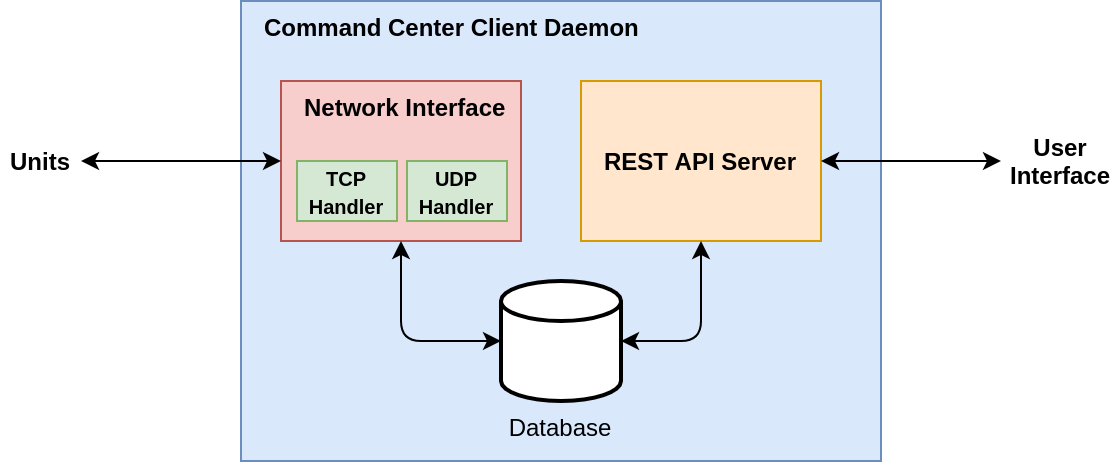
\includegraphics[width=\linewidth]{images/cmd-daemon.png}
    \caption{Command Center Client Daemon}
    \label{fig:cmd-daemon}
\end{figure} 

\subsubsection{Video Streamer}
For video streaming, we use HTTP Live Streaming (HLS) protocol. While video streaming is running at a unit, the command center client receives a metadata file and video segment files from the units continuously. The video streamer receives those files through the daemon, continuously updates the metadata, and stores the video segment files. In a dedicated media directory, the video streamer creates a directory per video stream per unit to store the video stream's metadata and video segment files and serve them to the user interface through a file server \acrshort{api} which maps endpoints paths to local file system paths.

When a video stream starts, the video streamer notifies the user interface through a \acrshort{sse}. The user interface reads the metadata to identify the available video segments, and starts fetching the video segments and displaying the video stream continuously through the file server \acrshort{api}. Figure \ref{fig:video-streamer} visualizes the data flow through the video streamer.

\begin{figure}[!htb]
    \centering
    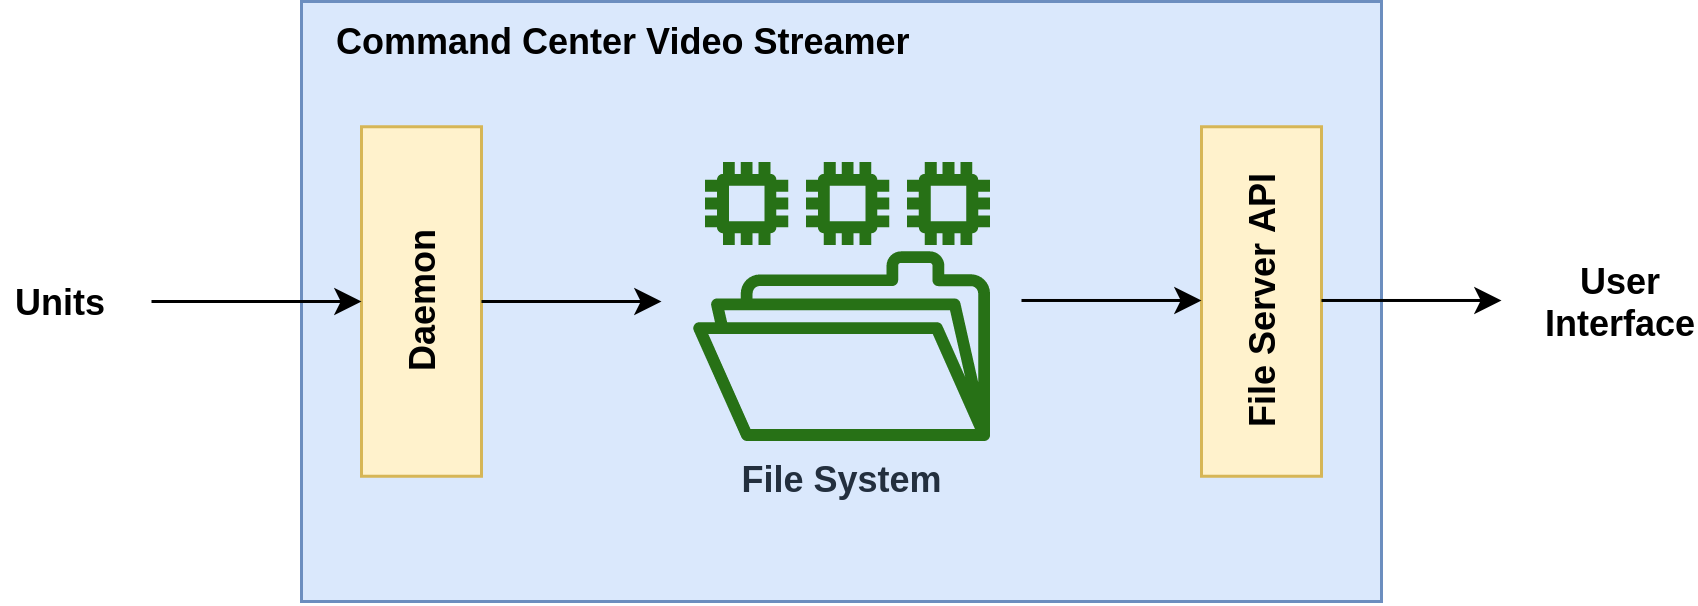
\includegraphics[width=\linewidth]{images/video-streamer.png}
    \caption{Video Streamer Data Flow}
    \label{fig:video-streamer}
\end{figure}

\subsubsection{User Interface}
The user interface in command center client allows operation leaders to manage and visualize units data, as well as record command audios and choose command codes that they want to send to these units.
There is two-way communication between the command center client daemon and the user interface. Data that recently arrived at the command center daemon is sent directly to the user interface using \acrfull{sse} to be visualized immediately to the operation leaders. While the data history is sent from command center daemon to user interface using \acrfull{rest} \acrshort{api} endpoints. 

Command center user interface is divided mainly into four pages: a login page, a map page, a units page, and finally a streams page. 
The login page is used to authenticate the operation leader to prevent masquerade attacks, as shown by Figure \ref{fig:cmd-ui-login}.

\begin{figure}[!htb]
    \centering
    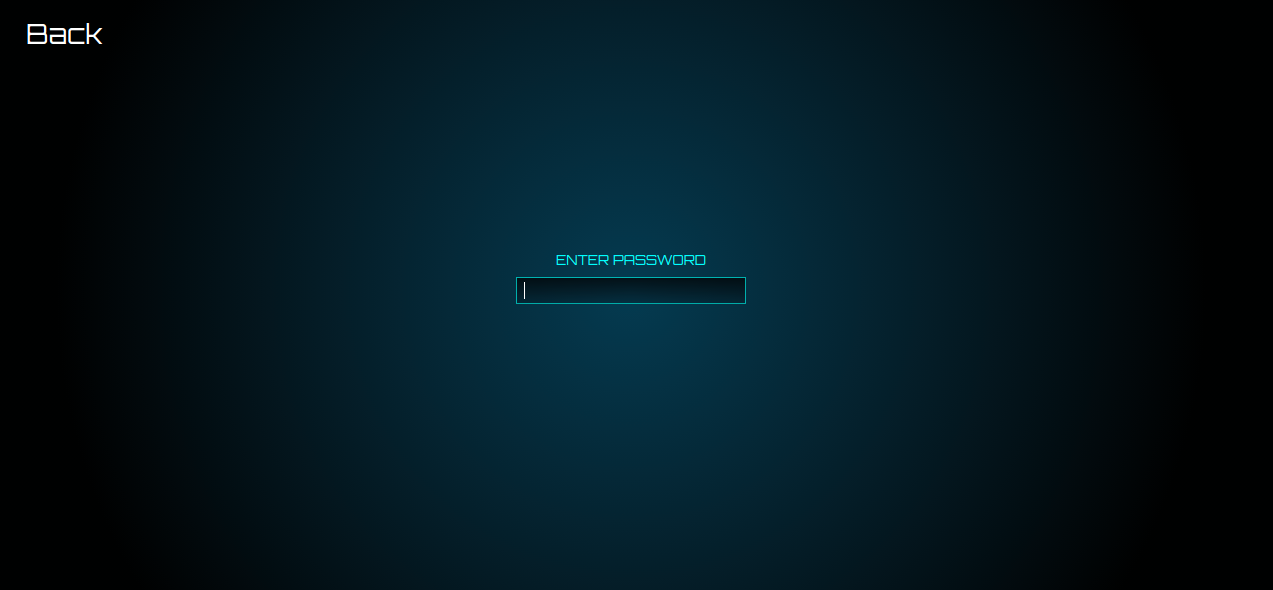
\includegraphics[width=15cm]{images/cmd-ui-login.png}
    \caption{\acrshort{cmd} \acrshort{ui} Login}
    \label{fig:cmd-ui-login}
\end{figure}


The map page is where the operation leader can view all nearby units' precise positions on a real map, as shown by Figure \ref{fig:cmd-ui-map-ch4}. Each unit is color-coded according to the group it belongs to, assisting the operation leader in analyzing group movements. When some unit sensor data indicates that this unit is in danger, or when some unit was inactive for more than two minutes and did not provide any sensor data during that time, the operation lead is informed. Any communications received from neighboring units are shown in a chat window. As soon as the data reaches the user interface, there will live update at the command center's screen. 

\begin{figure}[!htb]
    \centering
    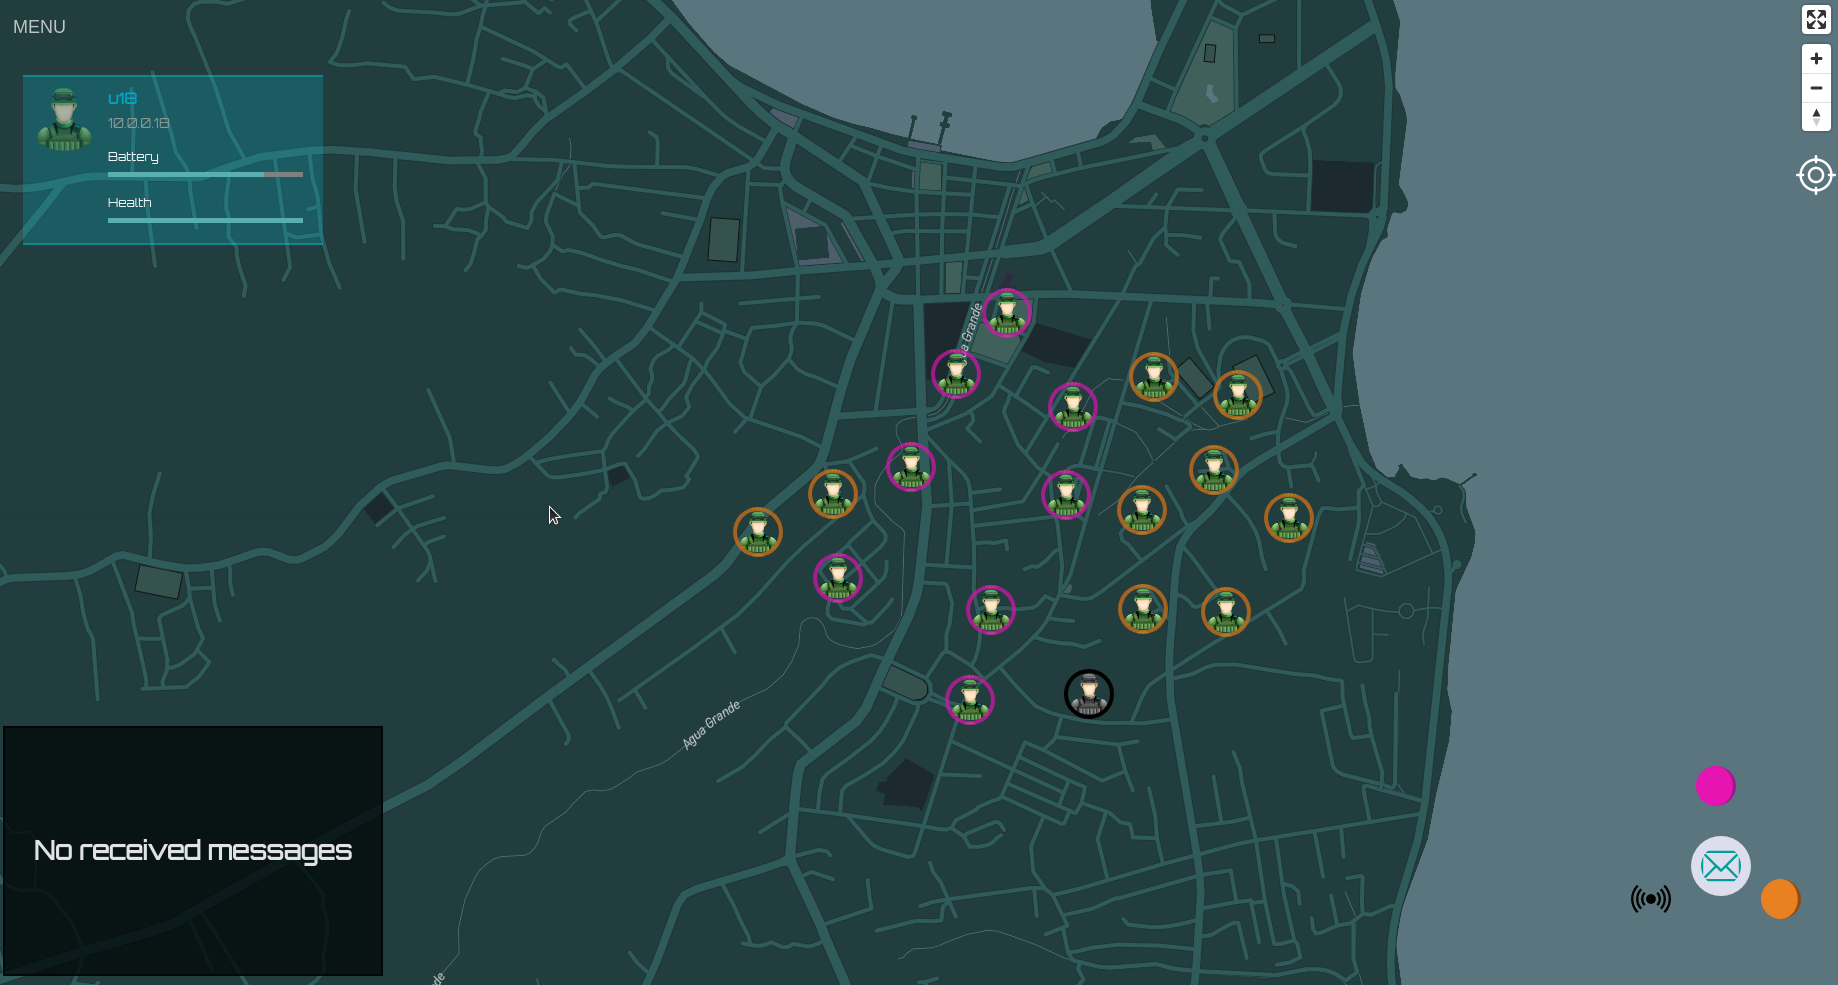
\includegraphics[width=15cm]{images/cmd-ui-map.png}
    \caption{\acrshort{cmd} \acrshort{ui} Map}
    \label{fig:cmd-ui-map-ch4}
\end{figure}


The operation leader can use the unit page (in Figure \ref{fig:cmd-ui-units-ch4}) to examine all of a unit's data history or send voice or message orders to it. All audios, videos, messages, position history, and sensors data of a unit are visible to the operation leader. 

\begin{figure}[!htb]
    \centering
    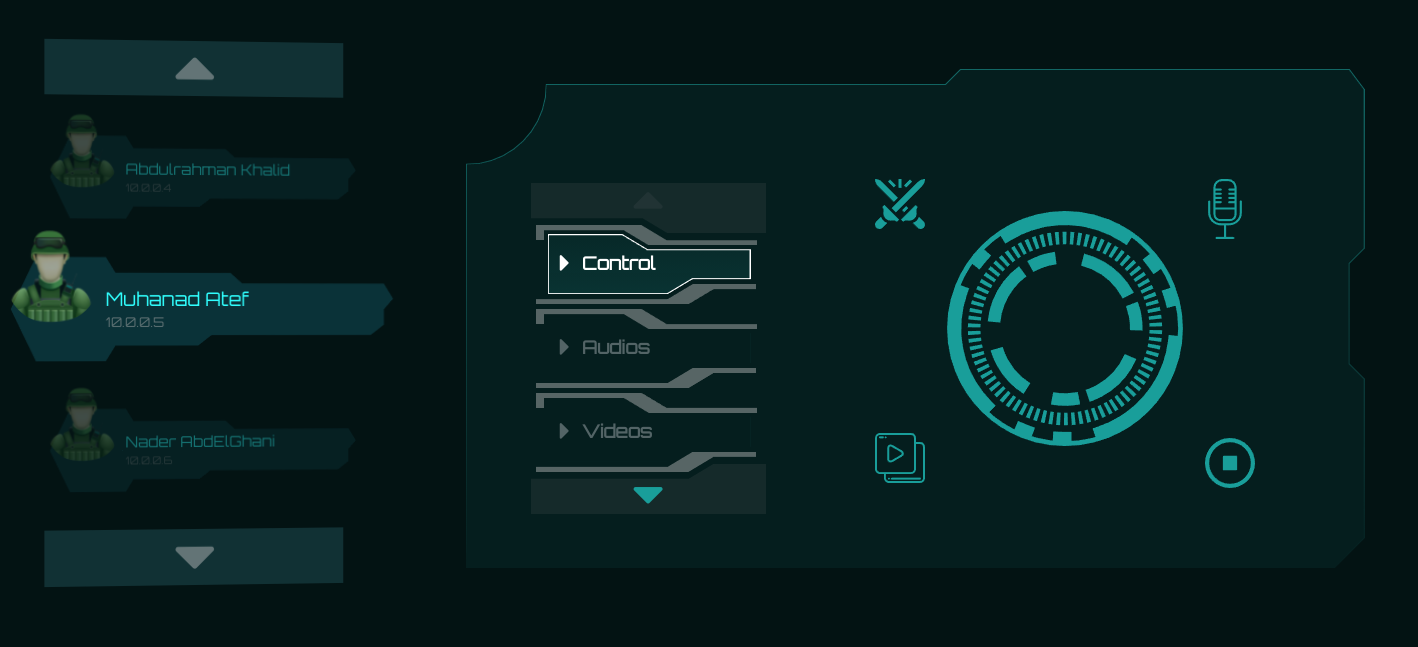
\includegraphics[width=15cm]{images/cmd-ui-units.png}
    \caption{\acrshort{cmd} \acrshort{ui} Units}
    \label{fig:cmd-ui-units-ch4}
\end{figure}


Finally, the operation leader may examine all live streams received from any nearby unit on the Streams page. This is shown by Figure \ref{fig:cmd-ui-streams-ch4}

\begin{figure}[!htb]
    \centering
    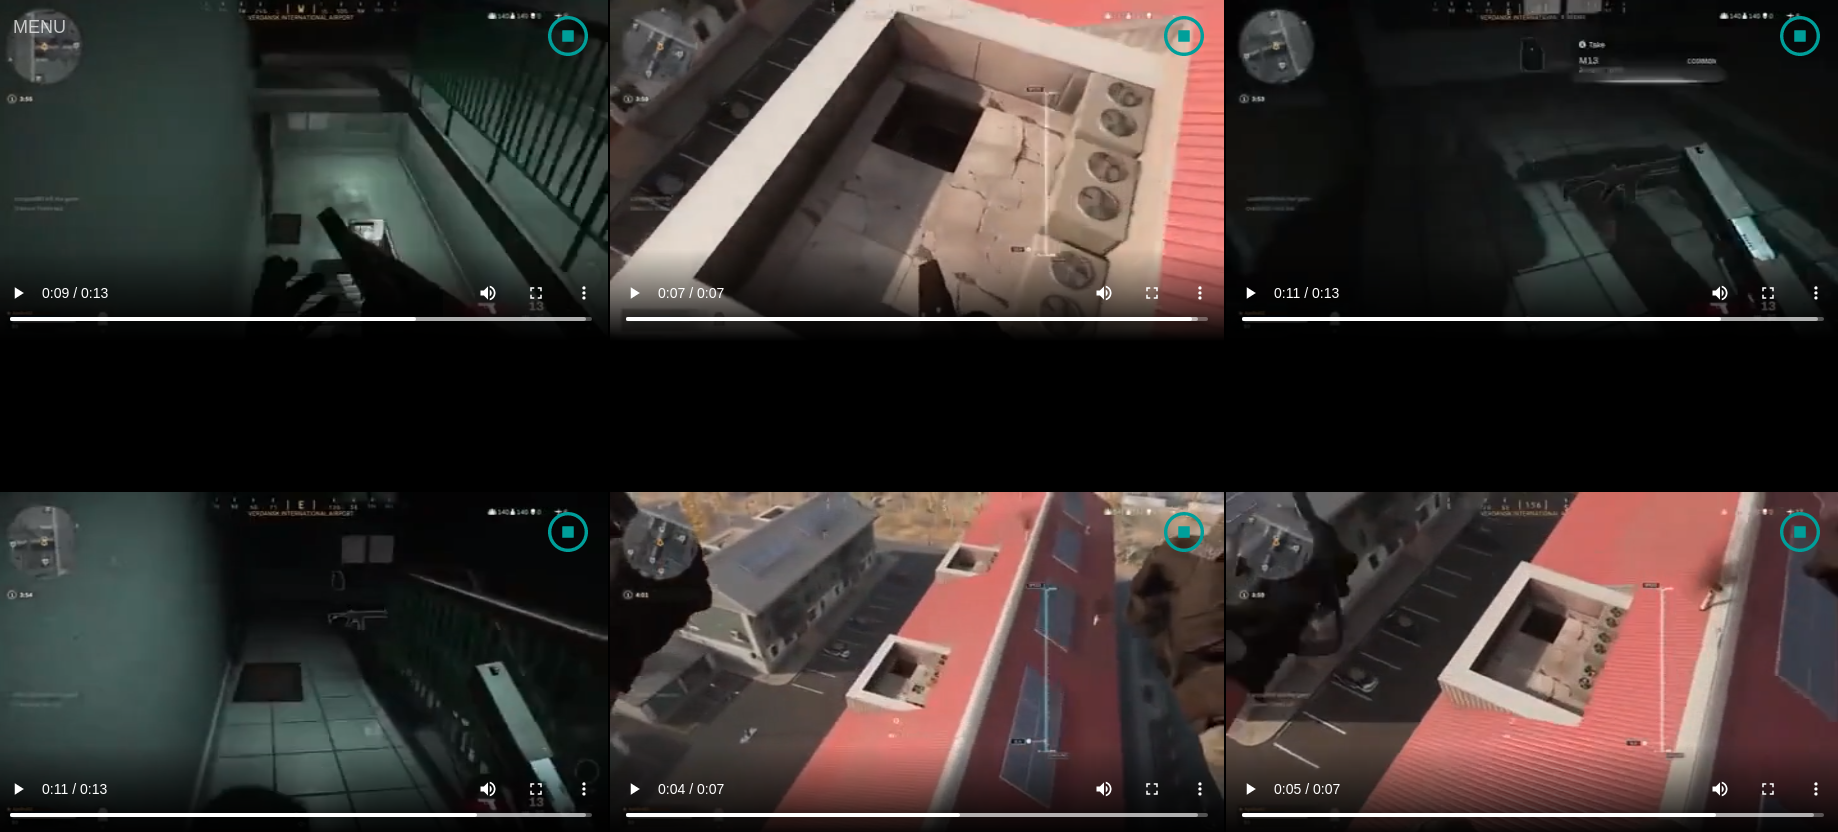
\includegraphics[width=15cm]{images/cmd-ui-streaming.png}
    \caption{\acrshort{cmd} \acrshort{ui} Streams}
    \label{fig:cmd-ui-streams-ch4}
\end{figure}


\section{Unit Client}
The unit client is the software that runs on the unit device, which is carried by the deployed soldiers and officers on the operation field.
More detail about the unit device in \ref{subsubsec:units-dev}.

\subsection{Functional Description}
\begin{itemize}[itemsep=1pt, topsep=5pt]
    \item Stream video from combat cameras to command center(s) only if the latter requested them. Video streaming terminates if the unit received an end-stream request, or the start request wasn’t refreshed after 1 minute.
    \item Stream the heartbeat and location of the device owner and their position every 10 seconds.
    \item Store all the recorded video and sensors (location and heartbeat) data locally.
    \item If the device user requested:
        \begin{itemize}[itemsep=1pt, topsep=5pt]
            \item Send audio messages from the microphone.
            \item Send code messages (every code has its predefined meaning.)
        \end{itemize}
    \item Receive audio messages from command centers into a queue.
    \item Play received audio messages from the queue instantly.
    \item Receive and show code messages.
\end{itemize}

\subsection{Modular Decomposition}
Figure \ref{fig:unit-modules} shows the modules of the unit client.

\begin{figure}[!htb]
    \centering
    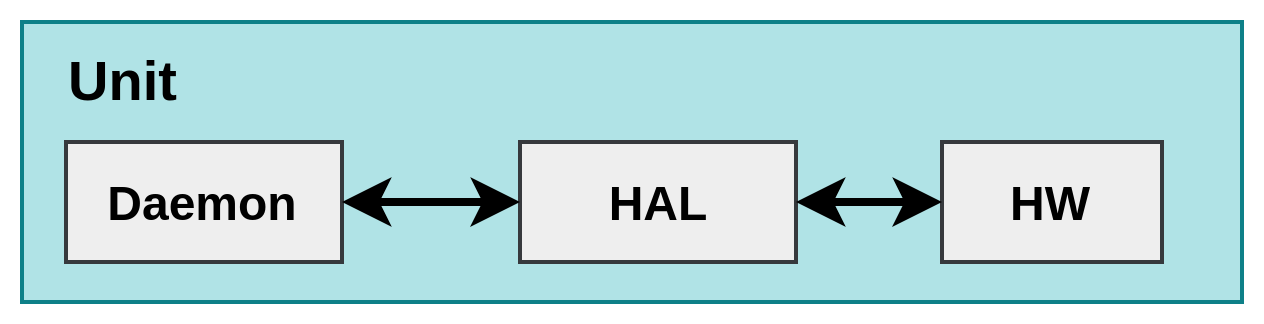
\includegraphics[width=11cm]{images/unit-modules.png}
    \caption{Unit Modules}
    \label{fig:unit-modules}
\end{figure}

The unit daemon implements the main state machine and logic of the unit.
It communicates with the daemon of the command center and transfers messages, whether they were audio or codes or streaming requests.

\acrfull{hal}, this abstracts the hardware, so we don't need to touch the unit client when porting to a different \acrshort{hw}.
It also serves the purpose of emulating the unit client \acrshort{hw} without the unit being aware of that.

\acrshort{hal} is responsible for streaming video from the camera source, or a video file in case we are testing.

\subsection{Design Constraints}
The unit runs on battery powered devices, so it needs minimal power and CPU consumption.

We lowered the CPU footprint by requiring \textit{FFmpeg} to generate only one level of quality for the video stream.
Also, we require that the command center should send stream request periodically to keep the stream. This is useful in case the command didn't want a stream, but the unit didn't receive its end video streaming request.
